%% bare_conf.tex
%% V1.3
%% 2007/01/11
%% by Michael Shell
%% See:
%% http://www.michaelshell.org/
%% for current contact information.
%%
%% This is a skeleton file demonstrating the use of IEEEtran.cls
%% (requires IEEEtran.cls version 1.7 or later) with an IEEE conference paper.
%%
%% Support sites:
%% http://www.michaelshell.org/tex/ieeetran/
%% http://www.ctan.org/tex-archive/macros/latex/contrib/IEEEtran/
%% and
%% http://www.ieee.org/

%%*************************************************************************
%% Legal Notice:
%% This code is offered as-is without any warranty either expressed or
%% implied; without even the implied warranty of MERCHANTABILITY or
%% FITNESS FOR A PARTICULAR PURPOSE! 
%% User assumes all risk.
%% In no event shall IEEE or any contributor to this code be liable for
%% any damages or losses, including, but not limited to, incidental,
%% consequential, or any other damages, resulting from the use or misuse
%% of any information contained here.
%%
%% All comments are the opinions of their respective authors and are not
%% necessarily endorsed by the IEEE.
%%
%% This work is distributed under the LaTeX Project Public License (LPPL)
%% ( http://www.latex-project.org/ ) version 1.3, and may be freely used,
%% distributed and modified. A copy of the LPPL, version 1.3, is included
%% in the base LaTeX documentation of all distributions of LaTeX released
%% 2003/12/01 or later.
%% Retain all contribution notices and credits.
%% ** Modified files should be clearly indicated as such, including  **
%% ** renaming them and changing author support contact information. **
%%
%% File list of work: IEEEtran.cls, IEEEtran_HOWTO.pdf, bare_adv.tex,
%%                    bare_conf.tex, bare_jrnl.tex, bare_jrnl_compsoc.tex
%%*************************************************************************

% *** Authors should verify (and, if needed, correct) their LaTeX system  ***
% *** with the testflow diagnostic prior to trusting their LaTeX platform ***
% *** with production work. IEEE's font choices can trigger bugs that do  ***
% *** not appear when using other class files.                            ***
% The testflow support page is at:
% http://www.michaelshell.org/tex/testflow/



% Note that the a4paper option is mainly intended so that authors in
% countries using A4 can easily print to A4 and see how their papers will
% look in print - the typesetting of the document will not typically be
% affected with changes in paper size (but the bottom and side margins will).
% Use the testflow package mentioned above to verify correct handling of
% both paper sizes by the user's LaTeX system.
%
% Also note that the "draftcls" or "draftclsnofoot", not "draft", option
% should be used if it is desired that the figures are to be displayed in
% draft mode.
%
\documentclass[conference]{IEEEtran}
% Add the compsoc option for Computer Society conferences.
%
% If IEEEtran.cls has not been installed into the LaTeX system files,
% manually specify the path to it like:
% \documentclass[conference]{../sty/IEEEtran}

% Some very useful LaTeX packages include:
% (uncomment the ones you want to load)

\newif\ifans\anstrue
% This is a package for drawing figures
% it is a part of standard latex 2e distribution
\usepackage{tikz}
\usetikzlibrary{shapes}
\usetikzlibrary{automata}

\usepackage[usenames,dvipsnames]{pstricks}
\usepackage{epsfig}
%\usepackage{pst-grad} % For gradients
%\usepackage{pst-plot} % For axes

\usepackage{palatino}
\RequirePackage{ifthen}
\usepackage{latexsym}
\RequirePackage{amsmath}
\RequirePackage{amsthm}
\RequirePackage{amssymb}
\RequirePackage{xspace}
\RequirePackage{graphics}
\usepackage{xcolor}
\usepackage{fullpage}
\usepackage{schemabloc}

\RequirePackage{textcomp}
\usepackage{keyval}
%\usepackage{listings}
\usepackage{xspace}
\usepackage{mathrsfs}
%\usepackage{textcomp}
%\usepackage{graphicx}
\usepackage{paralist}
\usepackage{amsmath,amssymb,url,listings,mathrsfs}
%\usepackage{pvs}
%\usepackage{supertabular,alltt,latexsym}
%\usepackage{multicol,multirow,epsfig}
%\usepackage[dvips, usenames]{color}
\usepackage{framed}
\usepackage{lipsum}
%\usepackage[dvipsnames]{color}



\definecolor{reddish}{rgb}{1,.8,0.8}
\definecolor{blueish}{rgb}{0.8,.8,1}
\definecolor{greenish}{rgb}{.8,1,0.8}
\definecolor{yellowish}{rgb}{1,1,.20}

\def\titleName{{Stability Analysis of Simplex Architecture Controlled Inverted Pendulum}}
\def\authorName{{Taylor Johnson}}

\usepackage[pdftex]{hyperref}
\hypersetup{
  pdftitle={\titleName},
  pdfauthor={\authorName},
  colorlinks=true,
  citecolor={blue},
  linkcolor = {blue},
  backref={true}
}

% marking changes

%\newcommand{\mitras}[1]{\textcolor{blue}{#1}}
\newcommand{\mitras}[1]{{#1}}
% for nomencl to produce page links
%\renewcommand*{\pagedeclaration}[1]{\unskip, \hyperpage{#1}}
%\renewcommand{\nomname}{List of Symbols and Functions}

\newcommand{\authcomment}[1]{\textbf{[[#1]]}}
\newcommand{\sayan}[1]{\textbf{[[#1]]}}


%FIXED SETS

%\newcommand{\Time}{{\sf T}}                     %time domain
\newcommand{\nnt}{{\sf T}^{\geq 0}}             %nonnegative time points
\newcommand{\post}{{\sf T}^{>0}}                %positive time points
\newcommand{\Variables}{{\sf V}}                %variables

\newcommand{\num}[1]{\relax\ifmmode \mathbb #1\else $\mathbb #1$\fi}
\newcommand{\nnnum}[1]{\relax\ifmmode 
  {\mathbb #1}_{\geq 0} \else ${\mathbb #1}_{\geq 0}$
  \fi}
\newcommand{\npnum}[1]{\relax\ifmmode 
  {\mathbb #1}_{\leq 0} \else ${\mathbb #1}_{\leq 0}$
  \fi}
\newcommand{\pnum}[1]{\relax\ifmmode 
  {\mathbb #1}_{> 0} \else ${\mathbb #1}_{> 0}$
  \fi}
\newcommand{\nnum}[1]{\relax\ifmmode 
  {\mathbb #1}_{< 0} \else ${\mathbb #1}_{< 0}$
  \fi}
\newcommand{\plnum}[1]{\relax\ifmmode 
  {\mathbb #1}_{+} \else ${\mathbb #1}_{+}$
  \fi}
\newcommand{\nenum}[1]{\relax\ifmmode 
  {\mathbb #1}_{-} \else ${\mathbb #1}_{-}$
  \fi}

\newcommand{\reals}{{\num R}}                    %reals
\newcommand{\nnreals}{{\nnnum R}}                    %nonnegative reals
\newcommand{\realsinfty}{{\num R} \cup \{\infty, -\infty\}}                    %nonnegative reals
\newcommand{\plreals}{{\plnum R}}                    %positive reals
\newcommand{\naturals}{{\num N}}                      %natural numbers
\newcommand{\integers}{{\num Z}}                      %integers
\newcommand{\rationals}{{\num Q}}                      %rationals
\newcommand{\nnrationals}{{\nnnum Q}}                   % nonnegative rationals
\newcommand{\Time}{{\num T}}  

% EXECUTIONS TRACES and FRAGS
\newcommand{\extb}[1]{\relax\ifmmode {\sf ExtBeh}_{#1} \else ${\sf ExtBeh}_{#1}$\fi} 
\newcommand{\tdists}[1]{\relax\ifmmode {\sf Tdists}_{#1} \else ${\sf Tdists}_{#1}$\fi} 

\newcommand{\exec}[1]{\relax\ifmmode {\sf Execs}_{#1} \else ${\sf Exec}_{#1}$\fi} 
\newcommand{\execf}[1]{\relax\ifmmode {\sf Execs}^*_{#1} \else ${\sf Exec}^*_{#1}$\fi} 
\newcommand{\execi}[1]{\relax\ifmmode {\sf Execs}^\omega_{#1} \else ${\sf Exec}^\omega_{#1}$\fi} 

\newcommand{\ctrace}[1]{\relax\ifmmode {\sf Ctraces}_{#1} \else ${\sf Ctraces}_{#1}$\fi} 

\newcommand{\trace}[1]{\relax\ifmmode {\sf Traces}_{#1} \else ${\sf Traces}_{#1}$\fi} 
\newcommand{\tracef}[1]{\relax\ifmmode {\sf Traces}^*_{#1} \else ${\sf Traces}^*_{#1}$\fi} 
\newcommand{\tracei}[1]{\relax\ifmmode {\sf Traces}^\omega_{#1} \else ${\sf Traces}^\omega_{#1}$\fi} 

\newcommand{\frag}[1]{\relax\ifmmode {\sf Frags}_{#1} \else ${\sf Frags}_{#1}$\fi} 
\newcommand{\fragf}[1]{\relax\ifmmode {\sf Frags}^*_{#1} \else ${\sf Frags}^*_{#1}$\fi} 
\newcommand{\fragi}[1]{\relax\ifmmode {\sf Frags}^\omega_{#1} \else ${\sf Frags}^\omega_{#1}$\fi} 

\newcommand{\reach}[1]{\relax\ifmmode {\sf Reach}_{#1} \else ${\sf Reach}_{#1}$\fi} 

\newcommand{\execs}{{\exec{}}}
\newcommand{\traces}{{\trace{}}}
\newcommand{\fragss}{{\frag{}}}

\newcommand{\fexecs}{{\execf{}}}
\newcommand{\ftraces}{{\tracef{}}}
\newcommand{\ffragss}{{\fragf{}}}

\newcommand{\iexecs}{{\execi{}}}
\newcommand{\itraces}{{\tracei{}}}
\newcommand{\ifragss}{{\fragi{}}}


\newenvironment{noqedproof}{\pf}{}
\newcommand{\pf}{\par\noindent{\bf Proof:}~}


% \newtheorem{theorem}{Theorem}[section]
% \newtheorem{lemma}[theorem]{Lemma}
% \newtheorem{corollary}[theorem]{Corollary}
 \newtheorem{claim}[theorem]{Claim}
\theoremstyle{definition}
% \newtheorem{definition}{Definition}[section]
 \renewcommand{\qed}{\hfill{\rule{2mm}{2mm}}\medskip}
 %\newenvironment{proof}{\pf}{\qed}
 \newtheorem{proposition}[theorem]{Proposition}
 \newtheorem{inv}[theorem]{Invariant}
 \newtheorem{remark}[theorem]{Remark}

 
 %\newenvironment{example}
 %{\refstepcounter{theorem} \vspace{2ex}\par\noindent
 %\textbf{Example}~\textbf{\thetheorem~}}{\qed}
 
\theoremstyle{remark}
 \newcounter{example}
% \newtheorem{example}{Example}[chapter]
% {\refstepcounter{theorem} \vspace{2ex}\par\noindent
% \textbf{Example}~\textbf{\theexampletheorem~}}{\qed}
 
 
 \def\examplenonum#1#2{
	\vspace{.15in}
	\noindent
	{\bf Example #1}{\em ~(continued)}{\bf .}
	{#2}{\qed}
	}
% 
% \renewcommand{\theequation}{\thesection.\arabic{equation}}
% \renewcommand{\thefigure}{\thesection.\arabic{figure}}
% \renewcommand{\thetable}{\thesection.\arabic{table}}
% \newcommand{\Section}[1]{\section{#1}%
%    \setcounter{equation}{0}\setcounter{figure}{0}\setcounter{table}{0}%
%    \setcounter{example}{0}}
% 
% \newenvironment{anotation}[1][Nancy]{\begin{quote}\small[[[#1]]]}{\normalsize\end{quote}}
% \newcommand{\ba}{\begin{anotation}}
% \newcommand{\ea}{\end{anotation}}
% 
% \newcommand{\bcb}{\chgbarbegin}
% \newcommand{\ecb}{\chgbarend}
% \chgbarwidth 1pt
% 
% \newcommand{\dec}{\ensuremath{{:}}}
% \newcommand{\eqdef}{\mathbin{::=}}
% \newcommand{\I}{{\ensuremath{\cap}}}



% OPERATIONS ON SETS, RELATIONS AND FUNCTIONS
\newcommand{\pow}[1]{{\bf P}(#1)} % powerset
\newcommand{\inverse}[1]{#1^{-1}}
\newcommand{\range}[1]{\ms{range{(#1)}}}
\newcommand{\domain}[1]{{\it dom}(#1)}
\newcommand{\type}[1]{\ms{type{(#1)}}}
\newcommand{\dtype}[1]{\ms{dtype{(#1)}}} % dynamic type
\newcommand{\restr}{\mathrel{\lceil}}
\newcommand{\proj}{\matrel{\lceil}}
\newcommand{\restrrange}{\mathrel{\downarrow}}
\newcommand{\point}[1]{\wp(#1)}     		%point trajectory



% HYBRID AUTOMATA
\def\A{{\cal A}} % HA
\def\B{{\cal B}} % HA
\def\C{{\cal C}} % HA
\def\D{{\cal D}} % set of discrete steps
\def\E{{\cal E}} % HA
\def\F{{\cal F}} % HA
\def\G{{\cal G}} % pieces of SHIOA
\def\H{{\cal H}} % HA
\def\I{{\cal I}} % environment sequence
\def\K{{\cal K}} % environment sequence
\def\M{{\cal M}} % Mode switching transitions
\def\O{{\cal O}} % outcome function
\def\P{{\cal P}} % set of modes
\def\Q{{\cal Q}} % set of modes
\def\R{{\cal R}} % relation
\def\S{{\cal S}} % set of trajectories
\def\T{{\cal T}} % set of trajectories
\def\V{{\cal V}} % Lyapunov function
\def\U{{\cal U}} % set of trajectories
\def\X{{\cal X}} % Lyapunov function
\def\Y{{\cal Y}} % set of trajectories
\def\KL{{\cal KL}}


% more special characters

\newcommand{\col}[1]{\relax\ifmmode \mathscr #1\else $\mathscr #1$\fi}

\def\statemodels{\col{S}}


% Names of actions, automata etc
\definecolor{HIOAcolor}{rgb}{0.776,0.22,0.07}
\newcommand{\HIOA}{\textcolor{HIOAcolor}{\tt HIOA\hspace{3pt}}}
\newcommand{\PVS}{\textcolor{HIOAcolor}{\tt PVS\hspace{3pt}}}
\newcommand{\PVSnogap}{\textcolor{HIOAcolor}{\tt PVS\hspace{1pt}}}
\newcommand{\HIOAbiggap}{\textcolor{HIOAcolor}{\tt HIOA\hspace{6pt}}}
\newcommand{\HIOAnogap}{\textcolor{HIOAcolor}{\tt HIOA}}
\newcommand{\anyrelation}{\lessgtr}

% Transformation for ADT
\newcommand{\SC}[2]{\relax\ifmmode {\tt Scount}(#1,#2) \else ${\tt Scount}(#1,#2)$\fi} 
\newcommand{\SCM}[2]{\relax\ifmmode {\tt Smin}(#1,#2) \else ${\tt Smin}(#1,#2)$\fi} 
\newcommand{\Aut}[1]{\relax\ifmmode {\tt Aut}(#1) \else ${\tt Aut}(#1)$\fi} 

\newcommand{\auto}[1]{{\operatorname{\mathsf{#1}}}}
\newcommand{\act}[1]{{\operatorname{\mathsf{#1}}}}
\newcommand{\smodel}[1]{{\operatorname{\mathsf{#1}}}}
\newcommand{\pvstheory}[1]{{\operatorname{\mathit{#1}}}}
%\newcommand{\auto}[1]{\relax\ifmmode \sf #1\else $\sf #1$\fi}
%\newcommand{\act}[1]{\relax\ifmmode \sf #1\else $\sf #1$\fi}


\newcommand{\Automaton}{{\bf automaton}}
\newcommand{\Asserts}{{\bf asserts}}
\newcommand{\Assumes}{{\bf assumes}}
\newcommand{\Backward}{{\bf backward}}
\newcommand{\By}{{\bf by}}
\newcommand{\Case}{{\bf case}}
\newcommand{\Choose}{{\bf  choose}}
\newcommand{\Components}{{\bf components}}
\newcommand{\Const}{{\bf const}}
\newcommand{\Converts}{{\bf converts}}
\newcommand{\Do}{{\bf do}}
\newcommand{\Eff}{{\bf eff}}
\newcommand{\Else}{{\bf else}}
\newcommand{\Elseif}{{\bf elseif}}
\newcommand{\Enumeration}{{\bf enumeration}}
\newcommand{\Ensuring}{{\bf ensuring}}
\newcommand{\Exempting}{{\bf exempting}}
\newcommand{\Fi}{{\bf fi}}
\newcommand{\For}{{\bf for}}
\newcommand{\Forward}{{\bf forward}}
\newcommand{\Freely}{{\bf freely}}
\newcommand{\From}{{\bf from}}
\newcommand{\Generated}{{\bf generated}}
\newcommand{\Local}{{\bf local}}
\newcommand{\Hidden}{{\bf hidden}}
\newcommand{\If}{{\bf if}}
\newcommand{\In}{{\bf in}}
\newcommand{\Implies}{{\bf implies}}
\newcommand{\Includes}{{\bf includes}}
\newcommand{\Introduces}{{\bf introduces}}
\newcommand{\Input}{{\bf input}}
\newcommand{\Kind}{{\bf kind}}
\newcommand{\Initially}{{\bf initially}}
\newcommand{\Internal}{{\bf internal}}
\newcommand{\Invariant}{{\bf invariant}}
\newcommand{\Od}{{\bf od}}
\newcommand{\Of}{{\bf of}}
\newcommand{\Output}{{\bf output}}
\newcommand{\Partitioned}{{\bf partitioned}}
\newcommand{\Pre}{{\bf pre}}
\newcommand{\Signature}{{\bf signature}}
\newcommand{\Simulation}{{\bf simulation}}
\newcommand{\Sort}{{\bf sort}}
\newcommand{\States}{{\bf states}}
\newcommand{\Tasks}{{\bf tasks}}
\newcommand{\Then}{{\bf then}}
\newcommand{\To}{{\bf to}}
\newcommand{\Trait}{{\bf trait}}
\newcommand{\Traits}{{\bf traits}}
\newcommand{\Transitions}{{\bf transitions}}
\newcommand{\Tuple}{{\bf tuple}}
\newcommand{\Type}{{\bf type}}
\newcommand{\Union}{{\bf union}}
\newcommand{\Uses}{{\bf uses}}
\newcommand{\Where}{{\bf where}}
\newcommand{\While}{{\bf while}}
\newcommand{\With}{{\bf with}}


% Spacing
\newcommand{\FFF}{\vspace{0.1in}}
\newcommand{\BBB}{\hspace{-0.1in}}


\newcommand{\deq}{\mathrel{\stackrel{\scriptscriptstyle\Delta}{=}}}


% systematic labels

\newcommand{\seclabel}[1]{\label{sec:#1}}
\newcommand{\secref}[1]{Section~\ref{sec:#1}}
\newcommand{\secreftwo}[2]{Sections~\ref{sec:#1}~and~\ref{sec:#2}}
\newcommand{\figlabel}[1]{\label{fig:#1}}
\newcommand{\figref}[1]{Figure~\ref{fig:#1}}
\newcommand{\figrefs}[2]{Figures~\ref{fig:#1} and~\ref{fig:#2}}
\newcommand{\applabel}[1]{\label{app:#1}}
\newcommand{\appref}[1]{Appendix~\ref{app:#1}}
\newcommand{\lnlabel}[1]{\label{line:#1}}
\newcommand{\lnrngref}[2]{lines~\ref{line:#1}--\ref{line:#2}\xspace}
\newcommand{\lnref}[1]{line~\ref{line:#1}\xspace}
\newcommand{\thmref}[1]{Theorem~\ref{thm:#1}\xspace}


% defs FROM ptioa PAPER


\newcommand{\remove}[1]{}
\newcommand{\salg}[1]{\relax\ifmmode {\mathcal F}_{#1}\else ${\mathcal F}_{#1}$\fi} 
\newcommand{\msp}[1]{\relax\ifmmode (#1, \salg{#1}) \else $(#1, \salg{#1})$\fi} 
\newcommand{\msprod}[2]{\relax\ifmmode ( #1 \times #2, \salg{#1} \otimes \salg{#2}) \else $(#1 \times #2, \salg{#1} \otimes \salg{#2})$\fi} 
\newcommand{\dist}[1]{\relax\ifmmode {\mathcal P}\msp{#1}
  \else ${\mathcal P}\msp{#1}$\fi} 
\newcommand{\subdist}[1]{\relax\ifmmode {\mathcal S}{\mathcal P}\msp{#1} 
  \else ${\mathcal S}{\mathcal P}\msp{#1}$\fi} 
\newcommand{\disc}[1]{\relax\ifmmode {\sf Disc}(#1)
  \else ${\sf Disc}(#1)$\fi} 

\newcommand{\Trajeq}{\relax\ifmmode {\mathcal R}_\T \else ${\mathcal R}_\T$\fi} 
\newcommand{\Acteq}{\relax\ifmmode {\mathcal R}_A \else ${\mathcal R}_A$\fi} 
\newcommand{\noop}{\relax\ifmmode \lambda \else $\lambda$\fi} 
\newcommand{\close}[1]{\relax\ifmmode \overline{#1} \else $\overline{#1}$\fi} 

\newcommand{\corrtasks}{\mathop{\mathsf {c}}}
\newcommand{\full}{\mathop{\mathsf {full}}}
%\newcommand{\fstate}{\mathop{\mathsf {fstate}}}
%\newcommand{\lstate}{\mathop{\mathsf {lstate}}}
\newcommand{\tdist}{\mathop{\mathsf {tdist}}}
\newcommand{\extbeh}{\mathop{\mathsf {extbeh}}}
%\newcommand{\apply}{\mathop{\mathsf {apply}}}
\newcommand{\apply}[2]{\mathop{\mathsf {apply}({#1},{#2})}}
%\newcommand{\applytwo}{\mathop{\mathsf {apply2}}}
\newcommand{\support}{\mathop{\mathsf {supp}}}
\newcommand{\relation}{\mathrel{R}}
\newcommand{\cone}{C}
%\newcommand{\tracef}{\mathord{\mathsf {trace}}}
\newcommand{\flatten}{\mathord{\mathsf {flatten}}}
\newcommand{\discrete}{\mathord{\mathsf {Disc}}}
\newcommand{\lift}[1]{\mathrel{{\mathcal L}(#1)}}
\newcommand{\expansion}[1]{\mathrel{{\mathcal E}(#1)}}
%End of commands added by Roberto on May, 12

%>> Ling, December 2005

\newcommand{\subdisc}{\operatorname{\mathsf {SubDisc}}}
\newcommand{\tran}{\operatorname{\mathsf {tran}}}
%\newcommand{\act}{\operatorname{\mathsf {act}}}

\renewcommand{\execs}{{\operatorname{\mathsf {Execs}}}}
\newcommand{\frags}{{\operatorname{\mathsf {Frags}}}}

\newcommand{\tracefnc}{{\operatorname{\mathsf {trace}}}}

\newcommand{\finite}{{\operatorname{\mathsf {finite}}}}
\newcommand{\hide}{{\operatorname{\mathsf {hide}}}}

\newcommand{\early}{{\operatorname{\mathsf {Early}}}}
\newcommand{\late}{{\operatorname{\mathsf {Late}}}}
\newcommand{\toss}{{\operatorname{\mathsf {Toss}}}}

\newcommand{\define}{:=}

\newcommand{\pc}{{\operatorname{\mathsf {counter}}}}
\newcommand{\chosen}{{\operatorname{\mathsf {chosen}}}}

\newcommand{\rand}{{\operatorname{\mathsf {random}}}}
\newcommand{\unif}{{\operatorname{\mathsf {unif}}}}

\newcommand{\ie}{i.e.,\xspace}
\newcommand{\Ie}{I.e.,\xspace}

\newcommand{\eg}{e.g.,\xspace}
\newcommand{\Eg}{E.g.,\xspace}

% IOA related stuff




\newcommand{\mybox}[3]{
  \framebox[#1][l]
  {
    \parbox{#2}
    {
      #3
    }
  }
}

\newcommand{\two}[4]{
  \parbox{.95\columnwidth}{\vspace{1pt} \vfill
    \parbox[t]{#1\columnwidth}{#3}%
    \parbox[t]{#2\columnwidth}{#4}%
  }}

\newcommand{\twosep}[4]{
  \parbox{\columnwidth}{\vspace{1pt} \vfill
    \parbox[t]{#1\columnwidth}{#3}%
   	\vrule width 0.2pt
    \parbox[t]{#2\columnwidth}{#4}%
  }}

\newcommand{\eqntwo}[4]{
  \parbox{\columnwidth}{\vspace{1pt} \vfill
    \parbox[t]{#1\columnwidth}{$ #3 $}
    \parbox[t]{#2\columnwidth}{$ #4 $}
  }}

\newcommand{\three}[6]{\vspace{1pt} \vfill
        \parbox{\columnwidth}{%
        \parbox[t]{#1\columnwidth}{#4}%
        \parbox[t]{#2\columnwidth}{#5}%
        \parbox[t]{#3\columnwidth}{#6}%
      }}

\newcommand{\tup}[1]
           {
             \relax\ifmmode
             \langle #1 \rangle
             \else $\langle$ #1 $\rangle$ \fi
           }

\newcommand{\lit}[1]{ \relax\ifmmode
                \mathord{\mathcode`\-="702D\sf #1\mathcode`\-="2200}
                \else {\it #1} \fi }


\newcommand{\figuresize}{\scriptsize}

\newcommand{\equationsize}{\footnotesize}

%\newcommand{\act}[1]{%
%  \relax\ifmmode
%                \mathord{\mathcode`\-="702D\sf #1\mathcode`\-="2200}%
%                \else
%                {\sf #1\/}%
%                \fi }


\lstdefinelanguage{ioa}{
  basicstyle=\figuresize,
  keywordstyle=\bf \figuresize,
  identifierstyle=\it \figuresize,
  emphstyle=\tt \figuresize,
  mathescape=true,
  tabsize=20,
%  tabsize=4,
  sensitive=false,
  columns=fullflexible,
  keepspaces=false,
  flexiblecolumns=true,
%  basewidth=0.5em,
  basewidth=0.05em,
  moredelim=[il][\rm]{//},
  moredelim=[is][\sf \figuresize]{!}{!},
  moredelim=[is][\bf \figuresize]{*}{*},
  keywords={automaton,and, 
  	 choose,const,continue, components,
  	 discrete, do,
  	 eff, external,else, elseif, evolve, end,
  	 fi,for, forward, from,
  	 hidden,
  	 in,input,internal,if,invariant, initially, imports,
     let,
     or, output, operators, od, of,
     pre,
     return,
     such,satisfies, stop, signature, simulation, 
     trajectories,trajdef, transitions, that,then, type, types, to, tasks,
     variables, vocabulary, 
     when,where, with,while},
  emph={set, seq, tuple, map, array, enumeration},   
   literate=
        {(}{{$($}}1
        {)}{{$)$}}1
        % LaTeX math symbols
        {\\in}{{$\in\ $}}1
        {\\preceq}{{$\preceq\ $}}1
        {\\subset}{{$\subset\ $}}1
        {\\subseteq}{{$\subseteq\ $}}1
        {\\supset}{{$\supset\ $}}1
        {\\supseteq}{{$\supseteq\ $}}1
        {\\forall}{{$\forall$}}1
        {\\le}{{$\le\ $}}1
        {\\ge}{{$\ge\ $}}1
        {\\gets}{{$\gets\ $}}1
        {\\cup}{{$\cup\ $}}1
        {\\cap}{{$\cap\ $}}1
        {\\langle}{{$\langle$}}1
        {\\rangle}{{$\rangle$}}1
        {\\exists}{{$\exists\ $}}1
        {\\bot}{{$\bot$}}1
        {\\rip}{{$\rip$}}1
        {\\emptyset}{{$\emptyset$}}1
        {\\notin}{{$\notin\ $}}1
        {\\not\\exists}{{$\not\exists\ $}}1
        {\\ne}{{$\ne\ $}}1
        {\\to}{{$\to\ $}}1
        {\\implies}{{$\implies\ $}}1
        % LSL symbols (one-character)
        {<}{{$<\ $}}1
        {>}{{$>\ $}}1
        {=}{{$=\ $}}1
        {~}{{$\neg\ $}}1
        {|}{{$\mid$}}1
        {'}{{$^\prime$}}1
        % LSL symbols (two characters)
        {\\A}{{$\forall\ $}}1
        {\\E}{{$\exists\ $}}1
        {\\/}{{$\vee\,$}}1
        {\\vee}{{$\vee\,$}}1
        {/\\}{{$\wedge\,$}}1
        {\\wedge}{{$\wedge\,$}}1
        {=>}{{$\Rightarrow\ $}}1
        {->}{{$\rightarrow\ $}}1
        {<=}{{$\Leftarrow\ $}}1
        {<-}{{$\leftarrow\ $}}1
%        {<=}{{$\leq$}}1
%        {>=}{{$\geq$}}1
        {~=}{{$\neq\ $}}1
        {\\U}{{$\cup\ $}}1
        {\\I}{{$\cap\ $}}1
        {|-}{{$\vdash\ $}}1
        {-|}{{$\dashv\ $}}1
        {<<}{{$\ll\ $}}2
        {>>}{{$\gg\ $}}2
        {||}{{$\|$}}1
%%       {\[\]}{{\[\,\]}}2 {\{\}}{{\{\,\}}}2
%%        {[}{{$\langle$}}1
%%        {]}{{$\rangle$}}1
        {[}{{$[$}}1
        {]}{{$\,]$}}1
        {[[}{{$\langle$}}1
        {]]]}{{$]\rangle$}}1
        {]]}{{$\rangle$}}1
        {<=>}{{$\Leftrightarrow\ $}}2
        {<->}{{$\leftrightarrow\ $}}2
        {(+)}{{$\oplus\ $}}1
        {(-)}{{$\ominus\ $}}1
        {_i}{{$_{i}$}}1
        {_j}{{$_{j}$}}1
        {_{i,j}}{{$_{i,j}$}}3
        {_{j,i}}{{$_{j,i}$}}3
        {_0}{{$_0$}}1
        {_1}{{$_1$}}1
        {_2}{{$_2$}}1
        {_n}{{$_n$}}1
        {_p}{{$_p$}}1
        {_k}{{$_n$}}1
        {-}{{$\ms{-}$}}1
        {@}{{}}0
        {\\delta}{{$\delta$}}1
        {\\R}{{$\R$}}1
        {\\Rplus}{{$\Rplus$}}1
        {\\N}{{$\N$}}1
        {\\times}{{$\times\ $}}1
        {\\tau}{{$\tau$}}1
        {\\alpha}{{$\alpha$}}1
        {\\beta}{{$\beta$}}1
        {\\gamma}{{$\gamma$}}1
        {\\ell}{{$\ell\ $}}1
        {--}{{$-\ $}}1
        {\\TT}{{\hspace{1.5em}}}3        
      }

\lstdefinelanguage{ioaNums}[]{ioa}
{
  numbers=left,
  numberstyle=\tiny,
  stepnumber=2,
  numbersep=4pt
%  firstnumber=1
}

\lstdefinelanguage{ioaNumsRight}[]{ioa}
{
  numbers=right,
  numberstyle=\tiny,
  stepnumber=2,
  numbersep=4pt
%  firstnumber=1
}

\newcommand{\ioa}{\lstinline[language=IOA]}

\lstnewenvironment{IOA}%
  {\lstset{language=IOA}}
  {}

\lstnewenvironment{IOANums}%
  {
  \if@firstcolumn
    \lstset{language=IOA, numbers=left, firstnumber=auto}
  \else
    \lstset{language=IOA, numbers=right, firstnumber=auto}
  \fi
  }
  {}

\lstnewenvironment{IOANumsRight}%
  {
    \lstset{language=IOA, numbers=right, firstnumber=auto}
  }
  {}

%\lstnewenvironment{IOA}%
%  {\lstset{language=ioaLang}
%   \csname lst@SetFirstLabel\endcsname}
%  {\csname lst@SaveFirstLabel\endcsname\vspace{-4pt}\noindent}

\newcommand{\figioa}[5]{
  \begin{figure}[#1]
      \hrule \F
      {\figuresize \bf #2}
      \lstinputlisting[language=ioaLang]{#5}
      \F \hrule \F
      \caption{#3}
      \label{fig: #4}
  \end{figure}
}

\newcommand{\linefigioa}[9]{

}

\newcommand{\twofigioa}[8]{
  \begin{figure}[#1]
    \hrule \F
    {\figuresize \bf #2} \\
    \two{#5}{#6}
    {
      \lstinputlisting[language=ioaLang]{#7}
    }
    {
      \lstinputlisting[language=ioaLang]{#8}
    }
    \F \hrule \F
    \caption{#3}
    \label{fig: #4}
  \end{figure}
}



\lstdefinelanguage{ioaLang}{%
  basicstyle=\ttfamily\small,
  keywordstyle=\rmfamily\bfseries\small,
  identifierstyle=\small,
%  commentline=\%,
  keywords={assumes,automaton,axioms,backward,bounds,by,case,choose,components,const,d,det,discrete,do,eff,else,elseif,ensuring,enumeration,evolve,fi,fire,follow,for,forward,from,hidden,if,in,%
    input,initially,internal,invariant,let, local,od,of,output,pre,schedule,signature,so,%
    simulation,states,variables, tasks, stop,tasks,that,then,to,trajdef,trajectory,trajectories,transitions,tuple,type,union,urgent,uses,when,where,while,yield},
  literate=
        % LaTeX math symbols
        {\\in}{{$\in$}}1
        {\\preceq}{{$\preceq$}}1
        {\\subset}{{$\subset$}}1
        {\\subseteq}{{$\subseteq$}}1
        {\\supset}{{$\supset$}}1
        {\\supseteq}{{$\supseteq$}}1
        {\\rho}{{$\rho$}}1
        {\\infty}{{$\infty$}}1
        % LSL symbols (one-character)
        {<}{{$<$}}1
        {>}{{$>$}}1
        {=}{{$=$}}1
        {~}{{$\neg$}}1 
        {|}{{$\mid$}}1
        {'}{{$^\prime$}}1
        % LSL symbols (two characters)
        {\\A}{{$\forall$}}1 {\\E}{{$\exists$}}1
        {\\/}{{$\vee$}}1 {/\\}{{$\wedge$}}1 
        {=>}{{$\Rightarrow$}}1 
        {->}{{$\rightarrow$}}1 
        {<=}{{$\leq$}}1 {>=}{{$\geq$}}1 {~=}{{$\neq$}}1
        {\\U}{{$\cup$}}1 {\\I}{{$\cap$}}1
        {|-}{{$\vdash$}}1 {-|}{{$\dashv$}}1
        {<<}{{$\ll$}}2 {>>}{{$\gg$}}2
        {||}{{$\|$}}1
%       {\[\]}{{\[\,\]}}2 {\{\}}{{\{\,\}}}2
        % LSL symbols (three or more characters)
        {<=>}{{$\Leftrightarrow$}}2 
        {<->}{{$\leftrightarrow$}}2
        {(+)}{{$\oplus$}}1
        {(-)}{{$\ominus$}}1
}

\lstdefinelanguage{bigIOALang}{%
  basicstyle=\ttfamily,
  keywordstyle=\rmfamily\bfseries,
  identifierstyle=,
%  commentline=\%,
  keywords={assumes,automaton,axioms,backward,by,case,choose,components,const,%
    d,det,discrete,do,eff,else,elseif,ensuring,enumeration,evolve,fi,for,forward,from,hidden,if,in%
    input,initially,internal,invariant,local,od,of,output,pre,schedule,signature,so,%
    tasks, simulation,states,stop,tasks,that,then,to,trajdef,trajectories,transitions,tuple,type,union,urgent,uses,when,where,yield},
  literate=
        % LaTeX math symbols
        {\\in}{{$\in$}}1
        {\\preceq}{{$\preceq$}}1
        {\\subset}{{$\subset$}}1
        {\\subseteq}{{$\subseteq$}}1
        {\\supset}{{$\supset$}}1
        {\\supseteq}{{$\supseteq$}}1
        % LSL symbols (one-character)
        {<}{{$<$}}1
        {>}{{$>$}}1
        {=}{{$=$}}1
        {~}{{$\neg$}}1 
        {|}{{$\mid$}}1
        {'}{{$^\prime$}}1
        % LSL symbols (two characters)
        {\\A}{{$\forall$}}1 {\\E}{{$\exists$}}1
        {\\/}{{$\vee$}}1 {/\\}{{$\wedge$}}1 
        {=>}{{$\Rightarrow$}}1 
        {->}{{$\rightarrow$}}1 
        {<=}{{$\leq$}}1 {>=}{{$\geq$}}1 {~=}{{$\neq$}}1
        {\\U}{{$\cup$}}1 {\\I}{{$\cap$}}1
        {|-}{{$\vdash$}}1 {-|}{{$\dashv$}}1
        {<<}{{$\ll$}}2 {>>}{{$\gg$}}2
        {||}{{$\|$}}1
%       {\[\]}{{\[\,\]}}2 {\{\}}{{\{\,\}}}2
        % LSL symbols (three or more characters)
        {<=>}{{$\Leftrightarrow$}}2 
        {<->}{{$\leftrightarrow$}}2
        {(+)}{{$\oplus$}}1
        {(-)}{{$\ominus$}}1
}


\lstnewenvironment{BigIOA}%
  {\lstset{language=bigIOALang,basicstyle=\ttfamily}
   \csname lst@SetFirstLabel\endcsname}
  {\csname lst@SaveFirstLabel\endcsname\vspace{-4pt}\noindent}

\lstnewenvironment{SmallIOA}%
  {\lstset{language=ioaLang,basicstyle=\ttfamily\scriptsize}
   \csname lst@SetFirstLabel\endcsname}
  %{\csname lst@SaveFirstLabel\endcsname\vspace{-4pt}\noindent}
  {\csname lst@SaveFirstLabel\endcsname\noindent}


\newcommand{\true}{\relax\ifmmode \mathit true \else \em true \/\fi}
\newcommand{\false}{\relax\ifmmode \mathit false \else \em false \/\fi}



\newcommand{\Real}{{\operatorname{\texttt{Real}}}}
\newcommand{\Bool}{{\operatorname{\texttt{Bool}}}}
\newcommand{\Char}{{\operatorname{\texttt{Char}}}}
\newcommand{\ioaInt}{{\operatorname{\texttt{Int}}}}
\newcommand{\ioaNat}{{\operatorname{\texttt{Nat}}}}
\newcommand{\ioaAugR}{{\operatorname{\texttt{AugmentedReal}}}}
\newcommand{\ioaString}{{\operatorname{\texttt{String}}}}
\newcommand{\Discrete}{{\operatorname{\texttt{Discrete}}}}
%\newcommand{\Bool}{{\operatorname{\texttt{Bool}}}}

%\newcommand{\lnot}{\neg}
%\newcommand{\land}{\wedge}
%\newcommand{\lor}{\vee}
\newcommand{\limplies}{\Rightarrow}
\newcommand{\liff}{\Leftrightarrow}

\newlength{\bracklen}
\newcommand{\sem}[1]{\settowidth{\bracklen}{[}
     [\hspace{-0.5\bracklen}[#1]\hspace{-0.5\bracklen}]}

\newcommand{\defaultArraystretch}{1.4}
\renewcommand{\arraystretch}{\defaultArraystretch}

\newcommand{\gS}{\mathcal{S}}
\newcommand{\gV}{\mathcal{V}}
\newcommand{\freevars}{\mathcal{FV}}

\newcommand{\gVspec}{\mathcal{V}_\mathit{spec}}
\newcommand{\gVa}{\mathcal{V}_\mathit{A}}
\newcommand{\gVsig}{\mathcal{V}_\mathit{sigs}}
\newcommand{\gVso}{\mathcal{V}_\mathit{sorts}}
\newcommand{\gVop}{\mathcal{V}_\mathit{ops}}
\newcommand{\sort}{\mathit{sort}}
\newcommand{\sig}{\mathit{sig}}
\newcommand{\id}{\mathit{id}}
\newcommand{\sigsep}{\lsl`->`}

%\newcommand{\T}{\mathit{true}}
%\newcommand{\F}{\mathit{false}}

\newcommand{\super}[2]{\ensuremath{\mathit{#1}^\mathit{#2}}}
\newcommand{\tri}[3]{\ensuremath{\mathit{#1}^\mathit{#2}_\mathit{#3}}}
\newcommand{\Assumptions}{\ensuremath{\mathit{Assumptions}}}
\newcommand{\actPred}[3][\pi]{\tri{P}{#2,#1}{#3}}
\newcommand{\actualTypes}[1]{\super{actualTypes}{#1}}
\newcommand{\actuals}[1]{\super{actuals}{#1}}
\newcommand{\autActVars}[2][\pi]{\vars{#2}{},\vars{#2,#1}{}}
\newcommand{\bracket}[2]{\mathit{#1}[\mathit{#2}]}
\newcommand{\compVars}[1]{\super{compVars}{#1}}
\newcommand{\context}{\mathit{context}}
\newcommand{\ensuring}[2]{\tri{ensuring}{#1}{#2}}
\newcommand{\initPred}[1]{\tri{P}{#1}{init}}
\newcommand{\initVals}[1]{\super{initVals}{#1}}
\newcommand{\initially}[2]{\tri{initially}{#1}{#2}}
\newcommand{\invPred}[2]{\tri{Inv}{#1}{#2}}
\newcommand{\knownVars}[1]{\super{knownVars}{#1}}
\newcommand{\localPostVars}[2]{\tri{localPostVars}{#1}{#2}}
\newcommand{\localVars}[2]{\tri{localVars}{#1}{#2}}
\newcommand{\locals}[1]{\bracket{Locals}{#1}}
\newcommand{\nam}[1]{\rho^{\mathit{#1}}}
\newcommand{\otherActPred}[3][\pi]{\otherTri{P}{#2,#1}{#3}}
\newcommand{\otherParams}[2]{\otherTri{params}{#1}{#2}}
\newcommand{\otherSub}[2]{\otherTri{\sigma}{#1}{#2}}
\newcommand{\otherTri}[3]{\tri{\smash{#1'}}{#2}{#3}}
\newcommand{\otherVars}[2]{\otherTri{vars}{#1}{#2}}
\newcommand{\params}[2]{\tri{params}{#1}{#2}}
\newcommand{\postVars}[1]{\super{postVars}{#1}}
\newcommand{\pre}[2]{\tri{Pre}{#1}{#2}}
\newcommand{\prog}[2]{\tri{Prog}{#1}{#2}}
\newcommand{\prov}[2]{\tri{Prov}{#1}{#2}}
\newcommand{\stateSorts}[1]{\super{stateSorts}{#1}}
\newcommand{\stateVars}[1]{\super{stateVars}{#1}}
\newcommand{\states}[1]{\bracket{States}{#1}}
\newcommand{\sub}[2]{\tri{\sigma}{#1}{#2}}
\newcommand{\sugActPred}[3][\pi]{\tri{P}{#2,#1}{#3,desug}}
\newcommand{\sugLocalVars}[2]{\ifthenelse{\equal{}{#2}}%
                             {\tri{localVars}{#1}{desug}}%
                             {\tri{localVars}{#1}{#2,desug}}}
\newcommand{\sugVars}[2]{\ifthenelse{\equal{}{#2}}%
                        {\tri{vars}{#1}{desug}}%
                        {\tri{vars}{#1}{#2,desug}}}
\newcommand{\cVars}[1]{\super{cVars}{#1}}

\newcommand{\vmap}{\dot{\varrho}}
\newcommand{\map}[2]{\tri{\vmap}{#1}{#2}}

\newcommand{\types}[1]{\super{types}{#1}}
\newcommand{\vars}[2]{\tri{vars}{#1}{#2}}

\newcommand{\subActPred}[3][\pi]{\sub{#2,#1}{#3}(\tri{P}{#2,#1}{#3,desug})}
\newcommand{\subLocalVars}[2]{\sub{#1}{#2}(\tri{localVars}{#1}{#2,desug})}

\newcommand{\dA}{\hat{A}}
\newcommand{\renameAction}[1]{\ensuremath{\rho_{#1}(\vars{\dA{#1},\pi}{})}}
\newcommand{\renameComponent}[1]{\ensuremath{\rho_{#1}\dA_{#1}}}

\newenvironment{Syntax}{\[\begin{subSyntax}}{\end{subSyntax}\]\vspace{-.3in}}
\newenvironment{subSyntax}{\begin{array}{l}}{\end{array}}
\newcommand{\w}[1]{\mbox{\hspace*{#1em}}}



%TIOA macros
% Script math symbol name
\newcommand{\ms}[1]{\ifmmode%
\mathord{\mathcode`-="702D\it #1\mathcode`\-="2200}\else%
$\mathord{\mathcode`-="702D\it #1\mathcode`\-="2200}$\fi}

%\newcommand{\domain}[1]{{\it dom}(#1)} % domain

% KEYWORDS 
\newcommand{\kw}[1]{{\bf #1}} 
\newcommand{\tcon}[1]{{\tt #1}} 
\newcommand{\syn}[1]{{\tt #1}} 
\newcommand{\pvskw}[1]{{\sc #1}} 
\newcommand{\pvsid}[1]{{\operatorname{\mathit{#1}}}}


% TIMED AUTOMATA
\def\A{{\cal A}} % TA
\def\B{{\cal B}} % TA
\def\D{{\cal D}} % set of discrete steps
\def\T{{\cal T}} % set of trajectories

% VALUATIONS
\newcommand{\vv}{{\bf v}}
\newcommand{\vw}{{\bf w}}
\newcommand{\vx}{{\bf x}}
\newcommand{\vy}{{\bf y}}
\newcommand{\va}{{\bf a}}
\newcommand{\vb}{{\bf b}}
\newcommand{\vq}{{\bf q}}
\newcommand{\vs}{{\bf s}}
\newcommand{\vm}{{\bf m}}

% Transitions and trajectory operations
\newcommand{\arrow}[1]{\mathrel{\stackrel{#1}{\rightarrow}}}
\newcommand{\sarrow}[2]{\mathrel{\stackrel{#1}{\rightarrow_{#2}}}}
\newcommand{\concat}{\mathbin{^{\frown}}} % concatenation
\newcommand{\paste}{\mathrel{\diamond}}

% AUTOMATA
%\def\A{{\cal A}}
%\def\B{{\cal B}}
%\def\T{{\cal T}} % set of trajectories

\def\CC{{\mathscr C}} % concatenation closure

% PVS STUFF

\lstdefinelanguage{pvs}{
  basicstyle=\tt \figuresize,
  keywordstyle=\sc \figuresize,
  identifierstyle=\it \figuresize,
  emphstyle=\tt \figuresize,
  mathescape=true,
  tabsize=20,
%  tabsize=4,
  sensitive=false,
  columns=fullflexible,
  keepspaces=false,
  flexiblecolumns=true,
%  basewidth=0.5em,
  basewidth=0.05em,
  moredelim=[il][\rm]{//},
  moredelim=[is][\sf \figuresize]{!}{!},
  moredelim=[is][\bf \figuresize]{*}{*},
  keywords={and, 
  	 begin,
  	 cases, const,
  	 do,
  	 external, else, exists, end, endcases, endif,
  	 fi,for, forall, from,
  	 hidden,
  	 in, if, importing,
     let, lambda, lemma,
     measure, 
     not,
     or, of,
     return, recursive,
     stop, 
     theory, that,then, type, types, type+, to, theorem,
     var,
     with,while},
  emph={nat, setof, sequence, eq, tuple, map, array, enumeration, bool, real, exp, nnreal, posreal},   
   literate=
        {(}{{$($}}1
        {)}{{$)$}}1
        % LaTeX math symbols
        {\\in}{{$\in\ $}}1
        {\\mapsto}{{$\rightarrow\ $}}1
        {\\preceq}{{$\preceq\ $}}1
        {\\subset}{{$\subset\ $}}1
        {\\subseteq}{{$\subseteq\ $}}1
        {\\supset}{{$\supset\ $}}1
        {\\supseteq}{{$\supseteq\ $}}1
        {\\forall}{{$\forall$}}1
        {\\le}{{$\le\ $}}1
        {\\ge}{{$\ge\ $}}1
        {\\gets}{{$\gets\ $}}1
        {\\cup}{{$\cup\ $}}1
        {\\cap}{{$\cap\ $}}1
        {\\langle}{{$\langle$}}1
        {\\rangle}{{$\rangle$}}1
        {\\exists}{{$\exists\ $}}1
        {\\bot}{{$\bot$}}1
        {\\rip}{{$\rip$}}1
        {\\emptyset}{{$\emptyset$}}1
        {\\notin}{{$\notin\ $}}1
        {\\not\\exists}{{$\not\exists\ $}}1
        {\\ne}{{$\ne\ $}}1
        {\\to}{{$\to\ $}}1
        {\\implies}{{$\implies\ $}}1
        % LSL symbols (one-character)
        {<}{{$<\ $}}1
        {>}{{$>\ $}}1
        {=}{{$=\ $}}1
        {~}{{$\neg\ $}}1
        {|}{{$\mid$}}1
        {'}{{$^\prime$}}1
        % LSL symbols (two characters)
        {\\A}{{$\forall\ $}}1
        {\\E}{{$\exists\ $}}1
        {\\/}{{$\vee\,$}}1
        {\\vee}{{$\vee\,$}}1
        {/\\}{{$\wedge\,$}}1
        {\\wedge}{{$\wedge\,$}}1
        {->}{{$\rightarrow\ $}}1
        {=>}{{$\Rightarrow\ $}}1
        {->}{{$\rightarrow\ $}}1
        {<=}{{$\Leftarrow\ $}}1
        {<-}{{$\leftarrow\ $}}1
%        {<=}{{$\leq$}}1
%        {>=}{{$\geq$}}1
        {~=}{{$\neq\ $}}1
        {\\U}{{$\cup\ $}}1
        {\\I}{{$\cap\ $}}1
        {|-}{{$\vdash\ $}}1
        {-|}{{$\dashv\ $}}1
        {<<}{{$\ll\ $}}2
        {>>}{{$\gg\ $}}2
        {||}{{$\|$}}1
%%       {\[\]}{{\[\,\]}}2 {\{\}}{{\{\,\}}}2
%%        {[}{{$\langle$}}1
%%        {]}{{$\rangle$}}1
        {[}{{$[$}}1
        {]}{{$\,]$}}1
        {[[}{{$\langle$}}1
        {]]]}{{$]\rangle$}}1
        {]]}{{$\rangle$}}1
        {<=>}{{$\Leftrightarrow\ $}}2
        {<->}{{$\leftrightarrow\ $}}2
        {(+)}{{$\oplus\ $}}1
        {(-)}{{$\ominus\ $}}1
        {_i}{{$_{i}$}}1
        {_j}{{$_{j}$}}1
        {_{i,j}}{{$_{i,j}$}}3
        {_{j,i}}{{$_{j,i}$}}3
        {_0}{{$_0$}}1
        {_1}{{$_1$}}1
        {_2}{{$_2$}}1
        {_n}{{$_n$}}1
        {_p}{{$_p$}}1
        {_k}{{$_n$}}1
        {-}{{$\ms{-}$}}1
        {@}{{}}0
        {\\delta}{{$\delta$}}1
        {\\R}{{$\R$}}1
        {\\Rplus}{{$\Rplus$}}1
        {\\N}{{$\N$}}1
        {\\times}{{$\times\ $}}1
        {\\tau}{{$\tau$}}1
        {\\alpha}{{$\alpha$}}1
        {\\beta}{{$\beta$}}1
        {\\gamma}{{$\gamma$}}1
        {\\ell}{{$\ell\ $}}1
        {--}{{$-\ $}}1
        {\\TT}{{\hspace{1.5em}}}3        
      }



\lstdefinelanguage{BigPVS}{
  basicstyle=\tt,
  keywordstyle=\sc,
  identifierstyle=\it,
  emphstyle=\tt ,
  mathescape=true,
  tabsize=20,
%  tabsize=4,
  sensitive=false,
  columns=fullflexible,
  keepspaces=false,
  flexiblecolumns=true,
%  basewidth=0.5em,
  basewidth=0.05em,
  moredelim=[il][\rm]{//},
  moredelim=[is][\sf \figuresize]{!}{!},
  moredelim=[is][\bf \figuresize]{*}{*},
  keywords={and, 
  	 begin,
  	 cases, const,
  	 do, datatype,
  	 external, else, exists, end, endif, endcases,
  	 fi,for, forall, from,
  	 hidden,
  	 in, if, importing,
     let, lambda, lemma,
     measure,
     not,
     or, of,
     return, recursive,
     stop, 
     theory, that,then, type, types, type+, to, theorem,
     var,
     with,while},
  emph={nat, setof, sequence, eq, tuple, map, array, first, rest, add, enumeration, bool, real, posreal, nnreal},   
   literate=
        {(}{{$($}}1
        {)}{{$)$}}1
        % LaTeX math symbols
        {\\in}{{$\in\ $}}1
        {\\mapsto}{{$\rightarrow\ $}}1
        {\\preceq}{{$\preceq\ $}}1
        {\\subset}{{$\subset\ $}}1
        {\\subseteq}{{$\subseteq\ $}}1
        {\\supset}{{$\supset\ $}}1
        {\\supseteq}{{$\supseteq\ $}}1
        {\\forall}{{$\forall$}}1
        {\\le}{{$\le\ $}}1
        {\\ge}{{$\ge\ $}}1
        {\\gets}{{$\gets\ $}}1
        {\\cup}{{$\cup\ $}}1
        {\\cap}{{$\cap\ $}}1
        {\\langle}{{$\langle$}}1
        {\\rangle}{{$\rangle$}}1
        {\\exists}{{$\exists\ $}}1
        {\\bot}{{$\bot$}}1
        {\\rip}{{$\rip$}}1
        {\\emptyset}{{$\emptyset$}}1
        {\\notin}{{$\notin\ $}}1
        {\\not\\exists}{{$\not\exists\ $}}1
        {\\ne}{{$\ne\ $}}1
        {\\to}{{$\to\ $}}1
        {\\implies}{{$\implies\ $}}1
        % LSL symbols (one-character)
        {<}{{$<\ $}}1
        {>}{{$>\ $}}1
        {=}{{$=\ $}}1
        {~}{{$\neg\ $}}1
        {|}{{$\mid$}}1
        {'}{{$^\prime$}}1
        % LSL symbols (two characters)
        {\\A}{{$\forall\ $}}1
        {\\E}{{$\exists\ $}}1
        {\\/}{{$\vee\,$}}1
        {\\vee}{{$\vee\,$}}1
        {/\\}{{$\wedge\,$}}1
        {\\wedge}{{$\wedge\,$}}1
        {->}{{$\rightarrow\ $}}1
        {=>}{{$\Rightarrow\ $}}1
        {->}{{$\rightarrow\ $}}1
        {<=}{{$\Leftarrow\ $}}1
        {<-}{{$\leftarrow\ $}}1
%        {<=}{{$\leq$}}1
%        {>=}{{$\geq$}}1
        {~=}{{$\neq\ $}}1
        {\\U}{{$\cup\ $}}1
        {\\I}{{$\cap\ $}}1
        {|-}{{$\vdash\ $}}1
        {-|}{{$\dashv\ $}}1
        {<<}{{$\ll\ $}}2
        {>>}{{$\gg\ $}}2
        {||}{{$\|$}}1
%%       {\[\]}{{\[\,\]}}2 {\{\}}{{\{\,\}}}2
%%        {[}{{$\langle$}}1
%%        {]}{{$\rangle$}}1
        {[}{{$[$}}1
        {]}{{$\,]$}}1
        {[[}{{$\langle$}}1
        {]]]}{{$]\rangle$}}1
        {]]}{{$\rangle$}}1
        {<=>}{{$\Leftrightarrow\ $}}2
        {<->}{{$\leftrightarrow\ $}}2
        {(+)}{{$\oplus\ $}}1
        {(-)}{{$\ominus\ $}}1
        {_i}{{$_{i}$}}1
        {_j}{{$_{j}$}}1
        {_{i,j}}{{$_{i,j}$}}3
        {_{j,i}}{{$_{j,i}$}}3
        {_0}{{$_0$}}1
        {_1}{{$_1$}}1
        {_2}{{$_2$}}1
        {_n}{{$_n$}}1
        {_p}{{$_p$}}1
        {_k}{{$_n$}}1
        {-}{{$\ms{-}$}}1
        {@}{{}}0
        {\\delta}{{$\delta$}}1
        {\\R}{{$\R$}}1
        {\\Rplus}{{$\Rplus$}}1
        {\\N}{{$\N$}}1
        {\\times}{{$\times\ $}}1
        {\\tau}{{$\tau$}}1
        {\\alpha}{{$\alpha$}}1
        {\\beta}{{$\beta$}}1
        {\\gamma}{{$\gamma$}}1
        {\\ell}{{$\ell\ $}}1
        {--}{{$-\ $}}1
        {\\TT}{{\hspace{1.5em}}}3        
      }

\lstdefinelanguage{pvsNums}[]{pvs}
{
  numbers=left,
  numberstyle=\tiny,
  stepnumber=2,
  numbersep=4pt
%  firstnumber=1
}

\lstdefinelanguage{pvsNumsRight}[]{pvs}
{
  numbers=right,
  numberstyle=\tiny,
  stepnumber=2,
  numbersep=4pt
%  firstnumber=1
}

\newcommand{\pvs}{\lstinline[language=PVS]}

\lstnewenvironment{BigPVS}%
  {\lstset{language=BigPVS}}
  {}

\lstnewenvironment{PVSNums}%
  {
  \if@firstcolumn
    \lstset{language=pvs, numbers=left, firstnumber=auto}
  \else
    \lstset{language=pvs, numbers=right, firstnumber=auto}
  \fi
  }
  {}

\lstnewenvironment{PVSNumsRight}%
  {
    \lstset{language=pvs, numbers=right, firstnumber=auto}
  }
  {}


\newcommand{\figpvs}[5]{
  \begin{figure}[#1]
      \hrule \F
      {\figuresize \bf #2}
      \lstinputlisting[language=pvs]{#5}
      \F \hrule \F
      \caption{#3}
      \label{fig: #4}
  \end{figure}
}

\newcommand{\linefigpvs}[9]{

}

\newcommand{\twofigpvs}[8]{
  \begin{figure}[#1]
    \hrule \F
    {\figuresize \bf #2} \\
    \two{#5}{#6}
    {
      \lstinputlisting[language=pvsLang]{#7}
    }
    {
      \lstinputlisting[language=pvsLang]{#8}
    }
    \F \hrule \F
    \caption{#3}
    \label{fig: #4}
  \end{figure}
}


\lstdefinelanguage{pvsproof}{
  basicstyle=\tt \figuresize,
  mathescape=true,
  tabsize=4,
  sensitive=false,
  columns=fullflexible,
  keepspaces=false,
  flexiblecolumns=true,
  basewidth=0.05em,
}

\newcommand{\Giant}{\fontsize{120}{130}\selectfont}

\newcommand{\CrazyBig}{\fontsize{200}{210}\selectfont}



% *** MISC UTILITY PACKAGES ***
%'
%\usepackage{ifpdf}
% Heiko Oberdiek's ifpdf.sty is very useful if you need conditional
% compilation based on whether the output is pdf or dvi.
% usage:
% \ifpdf
%   % pdf code
% \else
%   % dvi code
% \fi
% The latest version of ifpdf.sty can be obtained from:
% http://www.ctan.org/tex-archive/macros/latex/contrib/oberdiek/
% Also, note that IEEEtran.cls V1.7 and later provides a builtin
% \ifCLASSINFOpdf conditional that works the same way.
% When switching from latex to pdflatex and vice-versa, the compiler may
% have to be run twice to clear warning/error messages.






% *** CITATION PACKAGES ***
%
\usepackage{cite}
% cite.sty was written by Donald Arseneau
% V1.6 and later of IEEEtran pre-defines the format of the cite.sty package
% \cite{} output to follow that of IEEE. Loading the cite package will
% result in citation numbers being automatically sorted and properly
% "compressed/ranged". e.g., [1], [9], [2], [7], [5], [6] without using
% cite.sty will become [1], [2], [5]--[7], [9] using cite.sty. cite.sty's
% \cite will automatically add leading space, if needed. Use cite.sty's
% noadjust option (cite.sty V3.8 and later) if you want to turn this off.
% cite.sty is already installed on most LaTeX systems. Be sure and use
% version 4.0 (2003-05-27) and later if using hyperref.sty. cite.sty does
% not currently provide for hyperlinked citations.
% The latest version can be obtained at:
% http://www.ctan.org/tex-archive/macros/latex/contrib/cite/
% The documentation is contained in the cite.sty file itself.





% *** GRAPHICS RELATED PACKAGES ***
%
\ifCLASSINFOpdf
  % \usepackage[pdftex]{graphicx}
  % declare the path(s) where your graphic files are
  % \graphicspath{{../pdf/}{../jpeg/}}
  % and their extensions so you won't have to specify these with
  % every instance of \includegraphics
  % \DeclareGraphicsExtensions{.pdf,.jpeg,.png}
\else
  % or other class option (dvipsone, dvipdf, if not using dvips). graphicx
  % will default to the driver specified in the system graphics.cfg if no
  % driver is specified.
  % \usepackage[dvips]{graphicx}
  % declare the path(s) where your graphic files are
  % \graphicspath{{../eps/}}
  % and their extensions so you won't have to specify these with
  % every instance of \includegraphics
  % \DeclareGraphicsExtensions{.eps}
\fi
% graphicx was written by David Carlisle and Sebastian Rahtz. It is
% required if you want graphics, photos, etc. graphicx.sty is already
% installed on most LaTeX systems. The latest version and documentation can
% be obtained at: 
% http://www.ctan.org/tex-archive/macros/latex/required/graphics/
% Another good source of documentation is "Using Imported Graphics in
% LaTeX2e" by Keith Reckdahl which can be found as epslatex.ps or
% epslatex.pdf at: http://www.ctan.org/tex-archive/info/
%
% latex, and pdflatex in dvi mode, support graphics in encapsulated
% postscript (.eps) format. pdflatex in pdf mode supports graphics
% in .pdf, .jpeg, .png and .mps (metapost) formats. Users should ensure
% that all non-photo figures use a vector format (.eps, .pdf, .mps) and
% not a bitmapped formats (.jpeg, .png). IEEE frowns on bitmapped formats
% which can result in "jaggedy"/blurry rendering of lines and letters as
% well as large increases in file sizes.
%
% You can find documentation about the pdfTeX application at:
% http://www.tug.org/applications/pdftex





% *** MATH PACKAGES ***
%
%\usepackage[cmex10]{amsmath}
% A popular package from the American Mathematical Society that provides
% many useful and powerful commands for dealing with mathematics. If using
% it, be sure to load this package with the cmex10 option to ensure that
% only type 1 fonts will utilized at all point sizes. Without this option,
% it is possible that some math symbols, particularly those within
% footnotes, will be rendered in bitmap form which will result in a
% document that can not be IEEE Xplore compliant!
%
% Also, note that the amsmath package sets \interdisplaylinepenalty to 10000
% thus preventing page breaks from occurring within multiline equations. Use:
%\interdisplaylinepenalty=2500
% after loading amsmath to restore such page breaks as IEEEtran.cls normally
% does. amsmath.sty is already installed on most LaTeX systems. The latest
% version and documentation can be obtained at:
% http://www.ctan.org/tex-archive/macros/latex/required/amslatex/math/





% *** SPECIALIZED LIST PACKAGES ***
%
%\usepackage{algorithmic}
% algorithmic.sty was written by Peter Williams and Rogerio Brito.
% This package provides an algorithmic environment fo describing algorithms.
% You can use the algorithmic environment in-text or within a figure
% environment to provide for a floating algorithm. Do NOT use the algorithm
% floating environment provided by algorithm.sty (by the same authors) or
% algorithm2e.sty (by Christophe Fiorio) as IEEE does not use dedicated
% algorithm float types and packages that provide these will not provide
% correct IEEE style captions. The latest version and documentation of
% algorithmic.sty can be obtained at:
% http://www.ctan.org/tex-archive/macros/latex/contrib/algorithms/
% There is also a support site at:
% http://algorithms.berlios.de/index.html
% Also of interest may be the (relatively newer and more customizable)
% algorithmicx.sty package by Szasz Janos:
% http://www.ctan.org/tex-archive/macros/latex/contrib/algorithmicx/




% *** ALIGNMENT PACKAGES ***
%
%\usepackage{array}
% Frank Mittelbach's and David Carlisle's array.sty patches and improves
% the standard LaTeX2e array and tabular environments to provide better
% appearance and additional user controls. As the default LaTeX2e table
% generation code is lacking to the point of almost being broken with
% respect to the quality of the end results, all users are strongly
% advised to use an enhanced (at the very least that provided by array.sty)
% set of table tools. array.sty is already installed on most systems. The
% latest version and documentation can be obtained at:
% http://www.ctan.org/tex-archive/macros/latex/required/tools/


%\usepackage{mdwmath}
%\usepackage{mdwtab}
% Also highly recommended is Mark Wooding's extremely powerful MDW tools,
% especially mdwmath.sty and mdwtab.sty which are used to format equations
% and tables, respectively. The MDWtools set is already installed on most
% LaTeX systems. The lastest version and documentation is available at:
% http://www.ctan.org/tex-archive/macros/latex/contrib/mdwtools/


% IEEEtran contains the IEEEeqnarray family of commands that can be used to
% generate multiline equations as well as matrices, tables, etc., of high
% quality.


%\usepackage{eqparbox}
% Also of notable interest is Scott Pakin's eqparbox package for creating
% (automatically sized) equal width boxes - aka "natural width parboxes".
% Available at:
% http://www.ctan.org/tex-archive/macros/latex/contrib/eqparbox/





% *** SUBFIGURE PACKAGES ***
%\usepackage[tight,footnotesize]{subfigure}
% subfigure.sty was written by Steven Douglas Cochran. This package makes it
% easy to put subfigures in your figures. e.g., "Figure 1a and 1b". For IEEE
% work, it is a good idea to load it with the tight package option to reduce
% the amount of white space around the subfigures. subfigure.sty is already
% installed on most LaTeX systems. The latest version and documentation can
% be obtained at:
% http://www.ctan.org/tex-archive/obsolete/macros/latex/contrib/subfigure/
% subfigure.sty has been superceeded by subfig.sty.



%\usepackage[caption=false]{caption}
%\usepackage[font=footnotesize]{subfig}
% subfig.sty, also written by Steven Douglas Cochran, is the modern
% replacement for subfigure.sty. However, subfig.sty requires and
% automatically loads Axel Sommerfeldt's caption.sty which will override
% IEEEtran.cls handling of captions and this will result in nonIEEE style
% figure/table captions. To prevent this problem, be sure and preload
% caption.sty with its "caption=false" package option. This is will preserve
% IEEEtran.cls handing of captions. Version 1.3 (2005/06/28) and later 
% (recommended due to many improvements over 1.2) of subfig.sty supports
% the caption=false option directly:
%\usepackage[caption=false,font=footnotesize]{subfig}
%
% The latest version and documentation can be obtained at:
% http://www.ctan.org/tex-archive/macros/latex/contrib/subfig/
% The latest version and documentation of caption.sty can be obtained at:
% http://www.ctan.org/tex-archive/macros/latex/contrib/caption/




% *** FLOAT PACKAGES ***
%
%\usepackage{fixltx2e}
% fixltx2e, the successor to the earlier fix2col.sty, was written by
% Frank Mittelbach and David Carlisle. This package corrects a few problems
% in the LaTeX2e kernel, the most notable of which is that in current
% LaTeX2e releases, the ordering of single and double column floats is not
% guaranteed to be preserved. Thus, an unpatched LaTeX2e can allow a
% single column figure to be placed prior to an earlier double column
% figure. The latest version and documentation can be found at:
% http://www.ctan.org/tex-archive/macros/latex/base/



%\usepackage{stfloats}
% stfloats.sty was written by Sigitas Tolusis. This package gives LaTeX2e
% the ability to do double column floats at the bottom of the page as well
% as the top. (e.g., "\begin{figure*}[!b]" is not normally possible in
% LaTeX2e). It also provides a command:
%\fnbelowfloat
% to enable the placement of footnotes below bottom floats (the standard
% LaTeX2e kernel puts them above bottom floats). This is an invasive package
% which rewrites many portions of the LaTeX2e float routines. It may not work
% with other packages that modify the LaTeX2e float routines. The latest
% version and documentation can be obtained at:
% http://www.ctan.org/tex-archive/macros/latex/contrib/sttools/
% Documentation is contained in the stfloats.sty comments as well as in the
% presfull.pdf file. Do not use the stfloats baselinefloat ability as IEEE
% does not allow \baselineskip to stretch. Authors submitting work to the
% IEEE should note that IEEE rarely uses double column equations and
% that authors should try to avoid such use. Do not be tempted to use the
% cuted.sty or midfloat.sty packages (also by Sigitas Tolusis) as IEEE does
% not format its papers in such ways.





% *** PDF, URL AND HYPERLINK PACKAGES ***
%
%\usepackage{url}
% url.sty was written by Donald Arseneau. It provides better support for
% handling and breaking URLs. url.sty is already installed on most LaTeX
% systems. The latest version can be obtained at:
% http://www.ctan.org/tex-archive/macros/latex/contrib/misc/
% Read the url.sty source comments for usage information. Basically,
% \url{my_url_here}.





% *** Do not adjust lengths that control margins, column widths, etc. ***
% *** Do not use packages that alter fonts (such as pslatex).         ***
% There should be no need to do such things with IEEEtran.cls V1.6 and later.
% (Unless specifically asked to do so by the journal or conference you plan
% to submit to, of course. )


% correct bad hyphenation here
\hyphenation{op-tical net-works semi-conduc-tor}


\begin{document}
%
% paper title
% can use linebreaks \\ within to get better formatting as desired
\title{\titleName}


% author names and affiliations
% use a multiple column layout for up to three different
% affiliations
\author{\IEEEauthorblockN{Taylor Johnson}
\IEEEauthorblockA{Department of Electrical and Computer Engineering\\
University of Illinois at Urbana-Champaign\\
Urbana, Illinois 61801\\
Email: johnso99@illinois.edu}}
%\and
%\IEEEauthorblockN{Homer Simpson}
%\IEEEauthorblockA{Twentieth Century Fox\\
%Springfield, USA\\
%Email: homer@thesimpsons.com}
%\and
%\IEEEauthorblockN{James Kirk\\ and Montgomery Scott}
%\IEEEauthorblockA{Starfleet Academy\\
%San Francisco, California 96678-2391\\
%Telephone: (800) 555--1212\\
%Fax: (888) 555--1212}}

% conference papers do not typically use \thanks and this command
% is locked out in conference mode. If really needed, such as for
% the acknowledgment of grants, issue a \IEEEoverridecommandlockouts
% after \documentclass

% for over three affiliations, or if they all won't fit within the width
% of the page, use this alternative format:
% 
%\author{\IEEEauthorblockN{Michael Shell\IEEEauthorrefmark{1},
%Homer Simpson\IEEEauthorrefmark{2},
%James Kirk\IEEEauthorrefmark{3}, 
%Montgomery Scott\IEEEauthorrefmark{3} and
%Eldon Tyrell\IEEEauthorrefmark{4}}
%\IEEEauthorblockA{\IEEEauthorrefmark{1}School of Electrical and Computer Engineering\\
%Georgia Institute of Technology,
%Atlanta, Georgia 30332--0250\\ Email: see http://www.michaelshell.org/contact.html}
%\IEEEauthorblockA{\IEEEauthorrefmark{2}Twentieth Century Fox, Springfield, USA\\
%Email: homer@thesimpsons.com}
%\IEEEauthorblockA{\IEEEauthorrefmark{3}Starfleet Academy, San Francisco, California 96678-2391\\
%Telephone: (800) 555--1212, Fax: (888) 555--1212}
%\IEEEauthorblockA{\IEEEauthorrefmark{4}Tyrell Inc., 123 Replicant Street, Los Angeles, California 90210--4321}}




% use for special paper notices
%\IEEEspecialpapernotice{(Invited Paper)}




% make the title area
\maketitle


\begin{abstract}
%\boldmath
Switched controllers are being used frequently for control of complex systems.  However, they introduce new challenges for verification of stability, of which a great deal of work in the hybrid systems domain has been formalizing recently.  This work is a stability case study of the classical inverted pendulum, in this case controlled using the Simplex architecture of \cite{ShaACC1998}, combining to form a complete system as in \cite{SetoSha1999}.  The main result shown uses small-gain theorems to prove the stability of the system with regards to measurement delays.
\end{abstract}
% IEEEtran.cls defaults to using nonbold math in the Abstract.
% This preserves the distinction between vectors and scalars. However,
% if the conference you are submitting to favors bold math in the abstract,
% then you can use LaTeX's standard command \boldmath at the very start
% of the abstract to achieve this. Many IEEE journals/conferences frown on
% math in the abstract anyway.

% no keywords




% For peer review papers, you can put extra information on the cover
% page as needed:
% \ifCLASSOPTIONpeerreview
% \begin{center} \bfseries EDICS Category: 3-BBND \end{center}
% \fi
%
% For peerreview papers, this IEEEtran command inserts a page break and
% creates the second title. It will be ignored for other modes.
\IEEEpeerreviewmaketitle



\section{Introduction and Preliminaries}
% no \IEEEPARstart

The physical system in Figure ~\ref{fig:pendulumSystem} consists of a DC-motor driven cart and a pendulum attached to the cart, with the control goal of keeping the angle $\theta$ of the pendulum at $0^{\circ}$ measured from the vertical.  There is an additional control goal of moving the cart to a set point $x_s$ along the $x$-axis.

This system is described by the nonlinear form 
\begin{equation}
\dot{x}=f(x,u)
\label{eq:nonlinearSystem}
\end{equation}

However, we work with a linearized model of the form
\begin{equation}
\dot{x}=Ax+Bu
\label{eq:linearSystem}
\end{equation}
\begin{center}
\begin{figure}[h!]
	\scalebox{1} {
		\begin{pspicture}(0,-2.94)(6.12,2.94)
		\psframe[linewidth=0.04,dimen=outer](5.42,0.56)(1.08,-1.1)
		\pscircle[linewidth=0.04,dimen=outer](2.09,-1.57){0.47}
		\psline[linewidth=0.04cm](0.0,-2.02)(6.1,-2.02)
		\pscircle[linewidth=0.04,dimen=outer](4.14,-1.56){0.48}
		\psline[linewidth=0.04cm,linestyle=dotted,dotsep=0.16cm](3.02,2.86)(3.0,0.56)
		\psline[linewidth=0.08cm](3.02,0.52)(4.2,2.9)
		\usefont{T1}{ptm}{m}{n}
		\rput(3.4390626,2.3){\large $\theta$}
		\usefont{T1}{ptm}{m}{n}
		\rput(3.298125,-0.295){\large M}
		\usefont{T1}{ptm}{m}{n}
		\rput(4.4246874,1.72){\large m, l}
		\psline[linewidth=0.04cm](0.2,-2.06)(0.2,-2.84)
		\psline[linewidth=0.04cm,arrowsize=0.05291667cm 2.0,arrowlength=1.4,arrowinset=0.4]{->}(0.24,-2.4)(4.32,-2.4)
		\usefont{T1}{ptm}{m}{n}
		\rput(1.8825,-2.72){\large x}
	\end{pspicture}}
	\caption{Inverted Pendulum System}
	\label{fig:pendulumSystem}
\end{figure}
\end{center}
The linearization is justified after the system description.  There are four state variables, the cart position $x$, cart velocity $\dot{x}$, pendulum angle $\theta$, and pendulum velocity $\dot{\theta}$ (we will now denote $X$ as the state vector and $x$ as the position, seen together in Equation ~\ref{eq:stateMatrix}).  As the system has been implemented, it is subject to physical constraints.  The range of $x$ is between $\left[-0.7,0.7\right]$ meters (and the set point [$x_s$] range is between $\left[-0.5,0.5\right]$ meters), $\dot{x}$ is between $\left[-1.0,1.0\right]$ meters/second, $\theta$ is between $\left[-30,30\right]^{\circ}$, and $\dot{\theta}$ is unconstrained.  Note that in the real implementation, to account for errors due to linearization and estimation (seen later), the constraints are made more conservative, so $x-x_s$ is between $\left[-0.2,0.2\right]$ meters and $\theta$ is between $\left[-15,15\right]^{\circ}$.

\begin{equation}
X=\left[ \begin{array}{c} x_1 \\ x_{2} \\ x_3 \\ x_{4} \end{array} \right]=\left[ \begin{array}{cccc} x-x_s \\ \dot{x} \\ \theta \\ \dot{\theta} \end{array} \right]
\label{eq:stateMatrix}
\end{equation}

The system is stabilized by linear state feedback of the form $\dot{X}=\left(A+BK\right)X$.  The control input, $u$ is the armature voltage of the DC-motor ($V_a$) and is constrained between $\left[-4.96,4.96\right]$ volts.  Thus, due to this control constraint, it is necessary to look at the system in the form of $\dot{X}=AX+Bu$ at some points of the later analysis.

The primary linearizations to note are that we ignore static friction (with respect to the cart wheels and ground, and with respect to the pendulum arm and joint) and take the armature inductance ($L_a=18$ millihenries) to be $0$ henry hence reducing the order of the system by making the armature current state variable $I_a$ a function of $V_a$.  Without this simplification, two control states would be necessary.  The linearization is justified since the control objective is to stabilize the system in a neighborhood of the vertical equilibrium, defined in this coordinate system as $\theta=0^{\circ}$.

For the remainder of the paper, we work towards proving stability of the system, first in the classical Lyapunov sense, and then using newer small-gain theorem results to also discuss stability in the delayed system as in \cite{LiberzonQuantDelay2006} and \cite{SanfeliceTeel2005}.  Recent results using small-gain theorems allow us to prove stability of systems with delay by analyzing the stability of a simpler system without delay.  The idea is to treat the error introduced by the delay as a disturbance input with bounded-gain, allowing us to talk about input-to-state stability.  Using this, we can find the maximum delay the system can tolerate.  Despite the linearizations of the system model, the small-gain techniques apply to nonlinear systems and can also be used to analyze stability in the more general system model.

\section{System and Controller Models}

Figure ~\ref{fig:systemModel} shows a high-level view of the entire control system.  We now discuss each block individually.  We are using hybrid input-output automata to describe the blocks, and we assume the reader is familiar with such notation, but if not, \cite{lynchSV2003} or \cite{MitraPhd2007} can serve as references to the notation.

\begin{center}
\begin{figure}[h!]
	\begin{tikzpicture}[auto, node distance=2cm,>=latex']
			\tikzstyle{block} = [draw, fill=blue!20, rectangle, 
			    minimum height=3em, minimum width=6em]
			\tikzstyle{sum} = [draw, fill=blue!20, circle, node distance=1cm]
			\tikzstyle{input} = [coordinate]
			\tikzstyle{output} = [coordinate]
			\tikzstyle{pinstyle} = [pin edge={to-,thin,black}]
			
	    % We start by placing the blocks
	    \node [input, name=topleft] {};
	    \node [block, below of=topleft] (actuator) {Actuator};
	    \node [input, name=botleft, below of=actuator] {};
	    \node [block, right of=topleft] (plant) {Plant};
			\node [block, right of=botleft] (controller) {Controller};
			\node [input, name=center, below of=plant] {};
			\node [block, right of=center] (sensor) {Sensor};
			\node [input, name=topright, above of=sensor] {};
			\node [input, name=botright, below of=sensor] {};
	
			\draw [->] (topleft) -- (plant);
			\draw [-] (plant) -- (topright);
			\draw [->] (topright) -- node {$x\left(t\right)$, $\theta\left(t\right)$} (sensor);
			\draw [-] (sensor) -- node {$x\left(t-\tau\right)$, \\$\theta\left(t-\tau\right)$} (botright);
			\draw [->] (botright) -- (controller);
			\draw [-] (controller) -- (botleft);
			\draw [->] (botleft) -- node {$u\left(t-\tau\right)$} (actuator);
			\draw [-] (actuator) -- node {$u\left(t-\tau\right)$} (topleft);
	
	    % Once the nodes are placed, connecting them is easy. 
	%    \draw [draw,->] (input) -- node {$r$} (sum);
	%    \draw [->] (sum) -- node {$e$} (controller);
	%    \draw [->] (system) -- node [name=y] {$y$}(output);
	%    \draw [->] (y) |- (measurements);
	%    \draw [->] (measurements) -| node[pos=0.99] {$-$} node [near end] {$y_m$} (sum);
	\end{tikzpicture}
	\caption{System Model}
	\label{fig:systemModel}
\end{figure}
\end{center}

\subsection{Plant Model}

The plant model of the inverted pendulum is described in Figure ~\ref{fig:plant}, where the two input parameters to the automaton plant, $A:\Real^{4\times 4}$ and $B:\Real^{4\times 1}$, are defined as 
\begin{equation}
A=\left[ \begin{array}{cccc} 0 & 1 & 0 & 0 \\ 0 & -a_{22} & -a_{23} & a_{24} \\ 0 & 0 & 0 & 1 \\ 0 & a_{42} & a_{43} & -a_{44} \end{array} \right]
\label{eq:systemMatrix}
\end{equation}
and
\begin{equation}
B=\left[ \begin{array}{c} 0 \\ b_{2} \\ 0 \\ -b_{4} \end{array} \right]
\label{eq:inputMatrix}
\end{equation} where $a_{22}=\frac{4\bar{B}}{D_l}$, $a_{23}=\frac{3mg}{D_l}$, $a_{24}=\frac{6B_{\theta}}{lD_l}$, $a_{42}=\frac{6\bar{B}}{lD_l}$, $a_{43}=\frac{6\bar{M}g}{lD_l}$, $a_{44}=\frac{12\bar{M}B_{\theta}}{ml^2D_l}$, 
$b_2=\frac{4B_l}{D_l}$, and $b_4=\frac{6B_1}{lD_l}$, 
for $D_l=4\bar{M}-3m$, 
$\bar{B}=\frac{K_gB_m}{r^2}+\frac{K_g^2K_iK_b}{r^2R_a}$, 
$B_l=\frac{K_gK_i}{rR_a}$,
$\bar{M}=\frac{m+M+(K_gJ_m)}{r^2}$, and where  
$g$ is gravity,
$R_a$ is the armature resistance,
$r$ is the driving wheel radius,
$J_m$ is the motor rotor inertia,
$B_m$ is the motor's coefficient of viscous friction,
$B_{\theta}$ is the pendulum joint's coefficient of viscous friction,
$K_i$ is the motor torque constant,
$K_b$ is the motor back-e.m.f. constant,
$K_g$ is the gear ratio,
$M$ is the cart mass, 
$m$ is the pendulum mass, and
$l$ is the pendulum length.  After applying real values, the $A$ and $B$ matrices used are 
\begin{equation}
A=\left[ \begin{array}{cccc} 0 & 1 & 0 & 0 \\ 0 & -10.95 & -2.75 & 0.0043 \\ 0 & 0 & 0 & 1 \\ 0 & 24.92 & 28.58 & -0.044 \end{array} \right]
\label{eq:systemMatrixReal}
\end{equation} and
\begin{equation}
B=\left[ \begin{array}{c} 0 \\ 1.94 \\ 0 \\ -4.44 \end{array} \right]
\label{eq:inputMatrixReal}
\end{equation}

\begin{figure}[h!]
\centering
  \hrule
%  {\lstinputlisting[language=ioa,lastline=8]{Plant.hioa}}
%  {\lstinputlisting[language=ioa,firstline=9]{Plant.hioa}}
  {\lstinputlisting[language=ioa,firstline=1]{Plant.hioa}}
  \hrule
  \caption{Linearized Plant Model}
  \label{fig:plant}
\end{figure}

\subsection{Sensor Model}

The sensor model can be seen in Figure ~\ref{fig:sensor}, and is an analog-to-digital converter (ADC).  This is where the delay is introduced to the system in the form of measurement delay, primarily due to filtering.  Between the sensor and the controller there exists a low-pass filter which will introduce a delay between one and two sampling periods ($T_s=20$ milliseconds) long.  There is also nondeterministic delay introduced due to the ADC and controller not being perfectly synchronized.  The ADC is utilizing a sample-and-hold, which must be finished before the controller reads the value, but the time difference between when the sample-and-hold finishes and the controller reads the value is unknown, but is assumed to be certainly less than one sampling period ($T_s$) long.  The filter delay will be decreased by model-based state projection described later.

\begin{figure}[h!]
\centering
  \hrule
%  \two{.47}{.47}
%  {\lstinputlisting[language=ioa,lastline=11]{Sensor.hioa}}
%  {\lstinputlisting[language=ioa,firstline=12]{Sensor.hioa}}
	{\lstinputlisting[language=ioa,firstline=1]{Sensor.hioa}}
  \hrule
  \caption{Sensor}
  \label{fig:sensor}
\end{figure}

\subsection{Actuator Model}
The actuator model serves little purpose at the present time, but is included for completeness as seen in Figure ~\ref{fig:actuator}, and may be used in the future to model the quantization error and delay introduced by this block.  The actuator is a digital-to-analog converter (DAC), followed by a higher power voltage source to drive the DC motor.  As a note, the delay introduced by the actuator is in general quite small, such as the switching time of toggling a power MOSFET, usually on the order of a few microseconds.  In the case of our control cycle period of $20$ milliseconds, this is negligible.

\begin{figure}[h!]
\centering
  \hrule
%  \two{.47}{.47}
%  {\lstinputlisting[language=ioa,lastline=14]{Actuator.hioa}}
%  {\lstinputlisting[language=ioa,firstline=15]{Actuator.hioa}}
	{\lstinputlisting[language=ioa,firstline=1]{Actuator.hioa}}
  \hrule
  \caption{Actuator}
  \label{fig:actuator}
\end{figure}

\subsection{Controller Model}

The controller is implemented following the Simplex architecture of \cite{ShaACC1998}.  The Simplex architecture is built on the concept of analytic redundancy of \cite{Bodson1994}, in this case, that several controllers implement the same control objective with different performance.  There are three controllers in this architecture, a safety controller that can stabilize the system from the largest set of initial conditions but with poor performance, a baseline controller that has better performance than the safety controller but cannot stabilize from such a wide set of initial conditions, and an experimental controller that has the best performance but the smallest set of stabilizable initial conditions.  The usefulness of such an architecture could be in upgrades of real-time systems that cannot afford downtime even for maintenance, such as critical infrastructure.  In our case, the architecture is used to differentiate between the different sets of recoverable initial conditions and performance.  Each controller uses linear state feedback for stabilization, with the only difference being higher gains in the baseline and experimental controllers to stabilize faster, with the downside that they cannot recover from certain initial conditions that the safety controller can.  Thus, the system is described as 
\begin{equation}
\dot{X}=\left(A+BK_{\sigma}\right)X
\label{eq:linearStateFeedbackDiffEq}
\end{equation} where $K_{\sigma}$ is one of the safety, baseline, or experimental controller gains and the solution to this is 
\begin{equation}
X=e^{\left(A+BK_{\sigma}\right)t}X_{0}
\label{eq:linearStateFeedbackSolution}
\end{equation} where $X_0$ is an initial condition within the stabilizable region.

Note that, as only $\theta$ and $x$ are measurable, $\dot{\theta}$ and $\dot{x}$ are constructed by the first-order approximations $\dot{\theta}(t)=\frac{[\theta(t)-\theta(t-mT_s)]}{mT_s}$ and $\dot{x}(t)=\frac{[x(t)-x(t-mT_s)]}{mT_s}$, where $m$ is an integer greater than one (chosen as $2$ by experimentation).  In the safety, baseline, and experimental controller automata, this first-order approximation is accomplished by storing a buffer of previous sampled values.  It is more logical to do this computation here than in the sensor automaton as this calculation is done in the controllers of the implemented system.

\subsubsection{Discretization}

As the system is implemented in embedded software, the system model needs to be discretized.  In continuous-time the system solution is of Equation ~\ref{eq:linearStateFeedbackSolution}, while the discrete solution is of the form 
\begin{equation}
X\left(t_0\right)=FX\left(t_0-T_s\right)+Gu\left(t_0-T_s\right)
\label{eq:discreteSolution}
\end{equation}
where
\begin{equation}
F=e^{AT_s}
\label{eq:discreteLinearStateFeedbackSolutionF}
\end{equation}
and
\begin{equation}
G=\int^{T_s}_0 e^{A\tau}d\tau
\label{discreteLinearStateFeedbackSolutionG}
\end{equation}

To get back to linear state feedback form, take the control as 
\begin{equation}
u\left(t_0\right)=KX\left(t_0-T_s\right)
\label{discreteLinearStateFeedbackSolutionu}
\end{equation}

yielding the full form

\begin{equation}
X\left(t_0\right)=FX\left(t_0-T_s\right)+GBKX\left(t_0-2T_s\right)
\label{eq:discreteLinearStateFeedbackSolution}
\end{equation}

This allows easy state projection of the form in Equation ~\ref{eq:discreteLinearStateFeedbackSolutionProjection}, where $n$ is the number of sampling periods to project forward.

\begin{equation}
  X\left(t_0+nT_s\right)=
	\label{eq:discreteLinearStateFeedbackSolutionProjection}
\end{equation}
\begin{equation*}
  FX\left(t_0+\left(n-1\right)T_s\right)+GBKX\left(t_0-\left(n-2\right)T_s\right) 
\end{equation*}

%\begin{eqnarray}
%  \lefteqn{X\left(t_0+nT_s\right)= } \\
%  & & FX\left(t_0+\left(n-1\right)T_s\right)+GBKX\left(t_0-\left(n-2\right)T_s\right) 
%\label{eq:discreteLinearStateFeedbackSolutionProjection}
%\end{eqnarray}

This projection is done to reduce the error introduced from the various delays in the system, primarily the digital implementation delay (that we are measuring the present state at $t_0$ and controlling the next state at $t_0+T_s$) and the aforementioned filter delay.

\subsubsection{Feasible and Stabilizable Regions}

The feasible region is the region defined by the aforementioned state constraints, so looking at only the $X$ and $\dot{X}$ constraints would produce a rectangle.  While $\dot{\theta}$ is unconstrained, since $V_a$ is in fact constrained, a maximal value of $\dot{\theta}$ is generated.  The stabilizable region is the region within which a given controller can stabilize the system.  This region is determined by solving a linear matrix inequality (LMI) (see, e.g. \cite{Boyd94}) of the determinant maximization form proposed by Vandenberghe in \cite{Vand98}.  This paper utilizes the work of \cite{Yalmip} and \cite{Sdpt3} to solve the LMI and generate the stabilizable region for each controller.  The stabilizable region is inversely related to the magnitude of the gains, so larger gains produce a smaller stabilizable region.  Thus, as the safety controller's stabilizable region corresponds to the largest stabilizable region, all other controllers will have stabilizable regions that are subsets of the safety controller's region.  This makes intuitive sense, as larger gains will create larger oscillations in the solution, potentially causing the system to go outside of even the feasible region.

The stabilizable regions for $x$ and $\dot{x}$ of each controller are seen in Figure ~\ref{fig:stabRegionX} and the regions for $\theta$ and $\dot{\theta}$ of each controller are in Figure ~\ref{fig:stabRegionTheta}.  The switching controller described later utilizes these regions to determine which gains to use.  Solving the LMI problem gives a matrix $P_{\sigma}$ for each controller, where checking $X^TP_{\sigma}X<1$ shows which stabilizable region (for $\sigma\in\left[sc,bc,ec\right]$) the states are within currently.

\begin{figure}[htp]
\centering
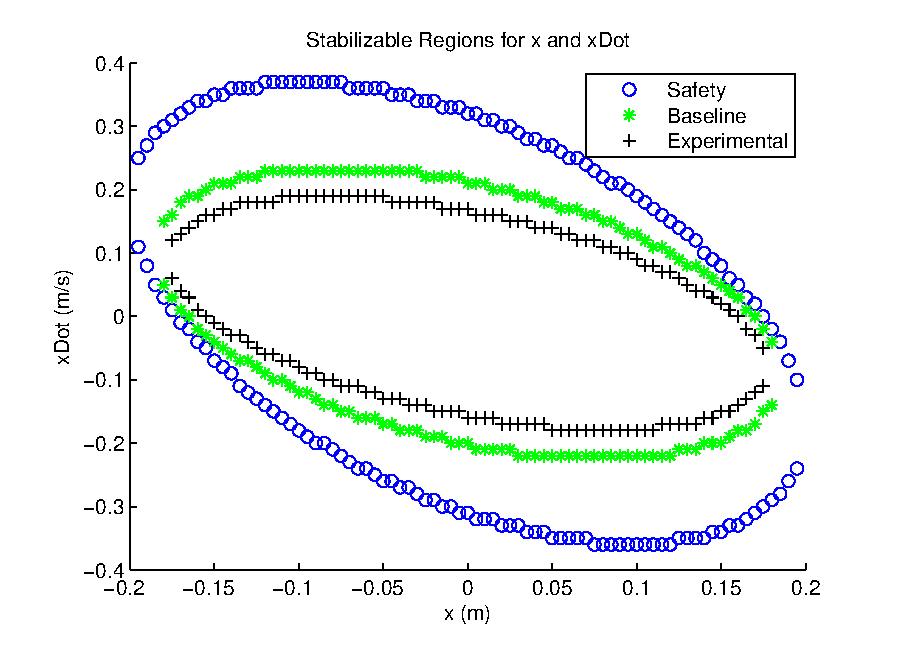
\includegraphics[width=250pt]{stabRegionX}
\caption{Stabilizable Region for $x$ and $\dot{x}$}\label{fig:stabRegionX}
\end{figure}

\begin{figure}[htp]
\centering
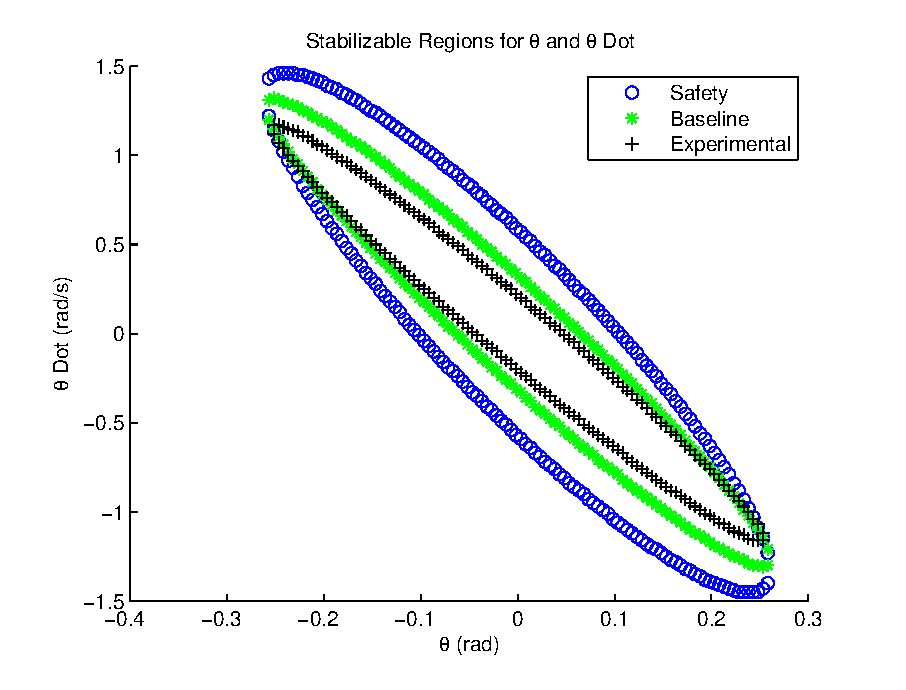
\includegraphics[width=250pt]{stabRegionTheta}
\caption{Stabilizable Region for $\theta$ and $\dot{\theta}$}\label{fig:stabRegionTheta}
\end{figure}


\subsubsection{Safety, Baseline, and Experimental Controllers}

\begin{figure}[h!]
\centering
  \hrule
%  \two{.47}{.47}
%  {\lstinputlisting[language=ioa,lastline=14]{SafetyController.hioa}}
%  {\lstinputlisting[language=ioa,firstline=15]{SafetyController.hioa}}
  {\lstinputlisting[language=ioa,firstline=1]{SafetyController.hioa}}
  \hrule
  \caption{Sigma Controller}
  \label{fig:safetyController}
\end{figure}

The safety, baseline, and experimental controllers are of the exact same form as the sigma controller in Figure ~\ref{fig:safetyController}, except to replace $\sigma\in\left[sc,bc,ec\right]$, noting that they use different gain matrices, $K_{sc}$ for the safety controller, $K_{bc}$ for the baseline controller, and $K_{ec}$ for the experimental controller.  We take the gains as follows to maximize the stability region for the safety controller, and to improve the performance for the baseline and experimental controllers.  In this form of control, increasing the gains will cause faster convergence with larger oscillations.  These increased oscillations for the baseline and experimental controllers could take the system outside of the largest stabilizable region, hence, their stabilizable regions must be subsets of the largest stabilizable region, each decreased by a factor to ensure that the largest oscillations do not take the system outside of the largest stabilizable region.

\begin{equation}
K_{sc}=\left[\begin{array}{c}6.0\\ 20.0\\ 60.0\\ 16.0\end{array}\right]
\end{equation}
\begin{equation}
K_{bc}=\left[\begin{array}{c}8.0\\ 32.0\\ 120.0\\ 12.0\end{array}\right]
\end{equation}
\begin{equation}
K_{ec}=\left[\begin{array}{c}10.0\\ 36.0\\ 140.0\\ 14.0\end{array}\right]
\end{equation}


\subsubsection{Switching Controller}

The switching controller determines which of the analytically redundant controllers to use for a given control cycle, based primarily on which stabilizable region the current and future states (determined by model-based state projection) of the system are within.  If the state measurements show the system to be within only the safety controller's stabilizable region, then the safety controller gains will be used.  Similarly, if the state is in the experimental stabilizable region, and will remain there for the next control cycle, the switching controller will utilize the experimental gains.  The specific controller to be used must also be ready.  The switching controller automaton can be seen in Figure ~\ref{fig:switchingController}.
After the switching controller receives the desired control value from one of the analytically redundant controllers, a corresponding ready flag is set.  Next, when the deadline is reached for the controller to output the new value to the motor, at $T_s$, the choice of controller is made.  While in general there is a matrix inequality to solve here, showing that $X^TPX<1$, it suffices to check that the control is within its constraints, as this model is linear, for an unconstrained control, it could stabilize the system from any initial condition in any amount of time.  Checking the matrix inequality could also be done easily (as one just has to check the norms of each state variable summed together are less than one), but this method removes unnecessary clutter from the automaton model.

\begin{figure}[h!]
\centering
  \hrule
%  \two{.47}{.47}
%  {\lstinputlisting[language=ioa,lastline=30]{SwitchingController.hioa}}
%  {\lstinputlisting[language=ioa,firstline=31]{SwitchingController.hioa}}
	{\lstinputlisting[language=ioa,firstline=1]{SwitchingController.hioa}}
  \hrule
  \caption{Switching Controller}
  \label{fig:switchingController}
\end{figure}

\section{Stability Analysis}

The stability analysis follows from classical Lyapunov stability (see, e.g. \cite{Chen1999} or \cite{Khalil2002}), and extends to the small-gain stability of systems with disturbances, such as in \cite{LiberzonQuantDelay2006}.

\subsection{Lyapunov Analysis}

From classical Lyapunov stability, we know that for linear time-invariant systems, if there exists some positive definite $P$ that solves the Lyapunov equation in Equation ~\ref{eq:lyapunovP} for some positive definite $Q$

\begin{equation}
PA+A^TP+Q=0
\label{eq:lyapunovP}
\end{equation} then the system is asymptotically stable and a function $V$ defined by Equation ~\ref{eq:lyapunovV} is a Lyapunov function.
\begin{equation}
V=X^TPX
\label{eq:lyapunovV}
\end{equation}

For our system, we have the following $P$ matrices 
\begin{equation}
P_{sc}=\left[ \begin{array}{cccc} 1.8030 & 2.3010 & 0.8447 & 0.3839 \\ 2.3010 &  10.0825 &   2.8171 &   1.4036 \\ 0.8447 &   2.8171 &   1.0109 &   0.4782 \\ 0.3839 &    1.4036 &   0.4782 &   0.2606 \end{array} \right]
%8.494 & 32.758 & 3.785  & 11.300 \\ 32.758 & 217.957  & 16.617  & 75.446 \\ 3.785  & 16.617   & 5.319   & 5.785 \\ 11.300  & 75.446   & 5.785  & 26.406
\label{eq:lyapSafeP}
\end{equation}
\begin{equation}
P_{bc}=\left[\begin{array}{cccc} 2.6836 &   2.7166 &   1.1849 &   0.5533 \\ 2.7166  & 10.0974 &   3.0287 &   1.4297 \\ 1.1849   & 3.0287 &   1.1695 &   0.5365 \\ 0.5533   & 1.4297 &   0.5365 &   0.2645\end{array}\right]
%10.623 &  48.942 &    6.132 &   16.600 \\ 48.942 &  350.558 &   25.975 &  119.079 \\
%6.132 &   25.975 &   44.397 &    8.836 \\ 16.600 & 119.079 &   8.836 &   42.101
\label{eq:lyapBaseP}
\end{equation}
\begin{equation}
P_{ec}=\left[\begin{array}{cccc} 1.6987 &   1.8877 &   0.7664 &   0.3461 \\ 1.8877 &   8.8812 &   2.5537 &   1.1747\\ 0.7664 &   2.5537 &   0.9601 &   0.4318\\ 0.3461 &   1.1747 &   0.4318 &   0.2050\end{array}\right]
%10.183 &   45.835 &    5.660 &   15.507 \\45.835 &  332.254 &   22.748 &  112.560 \\ 5.660 &   22.748 &   36.583 &    7.718 \\ 15.507 &  112.560 &    7.718 &   39.2890
\label{eq:lyapExpP}
\end{equation}
and then the corresponding Lyapunov functions $V_{sc}=X^TP_{sc}X$, $V_{bc}=X^TP_{bc}X$, and $V_{ec}=X^TP_{ec}X$.  Figures ~\ref{fig:lyapSafe}, ~\ref{fig:lyapBase}, and ~\ref{fig:lyapExp} show the Lyapunov functions along the system trajectory from initial conditions of $X_{0}=\left[\begin{array}{cccc} -0.170 & 0.130 & -0.258 & 1.170 \end{array}\right]^T$.

\begin{figure}[htp]
\centering
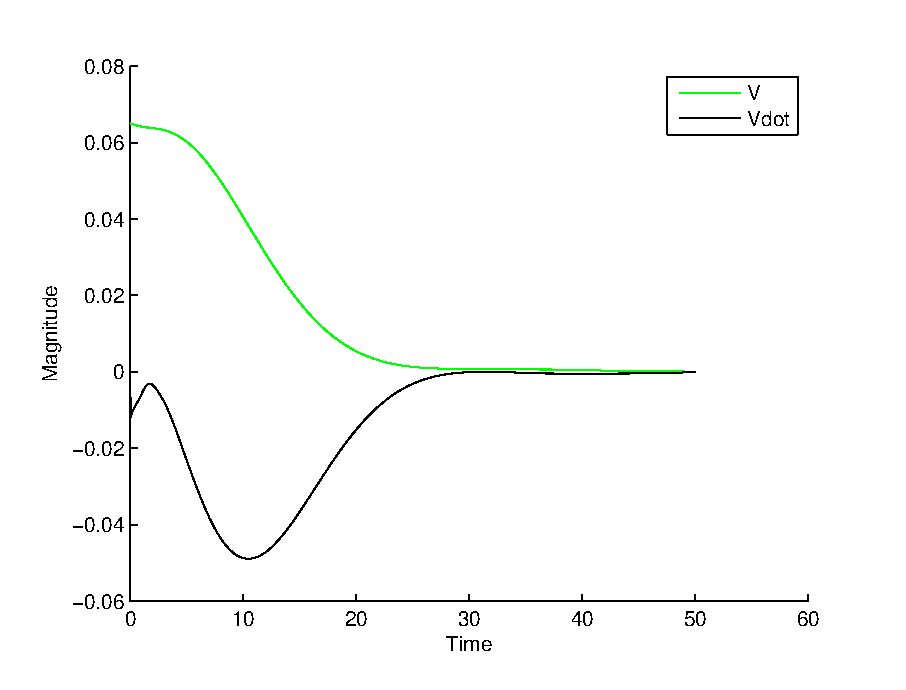
\includegraphics[width=250pt]{lyapSafe}
\caption{Lyapunov Function for Safety Controller}\label{fig:lyapSafe}
\end{figure}

\begin{figure}[htp]
\centering
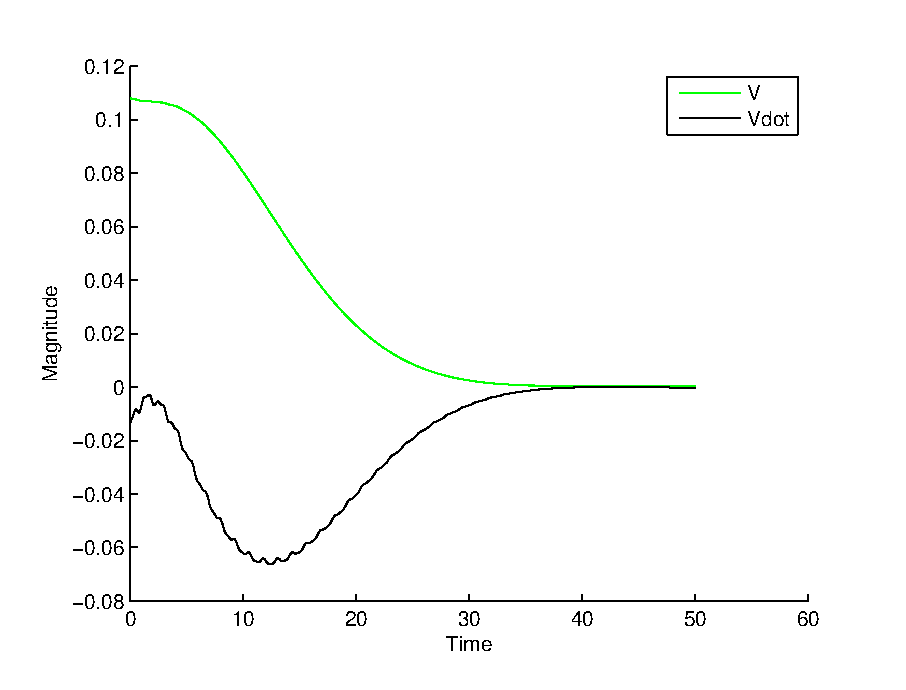
\includegraphics[width=250pt]{lyapBase}
\caption{Lyapunov Function for Baseline Controller}\label{fig:lyapBase}
\end{figure}

\begin{figure}[htp]
\centering
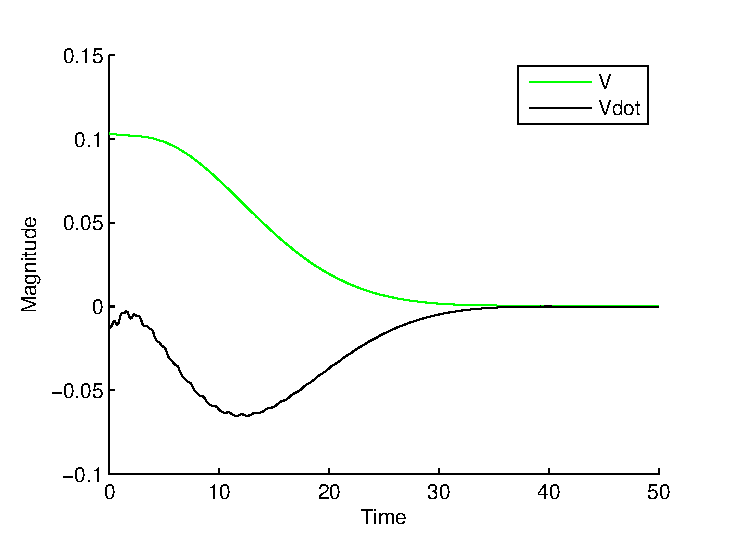
\includegraphics[width=250pt]{lyapExp}
\caption{Lyapunov Function for Experimental Controller}\label{fig:lyapExp}
\end{figure}

\subsection{Small-Gain Theorems}

Small-gain theorems allow us to bound the error introduced by the delay to talk about a system without delay, and instead with a disturbance injection.  Writing the delayed control as 
\begin{equation}
u\left(t\right)=KX\left(t-\tau\right)=KX\left(t\right)+\theta\left(t\right)
\end{equation} where $\theta\left(t\right)=KX\left(t-\tau\right)-KX\left(t\right)$ is the error from delay.

Now writing the system model again with this delay error as a disturbance input we have 
\begin{equation}
\dot{X}\left(t\right)=\left(A+BK\right)X\left(t\right)+B\theta\left(t\right)
\end{equation}

The Lyapunov function time-derivative changes in the form of 
\begin{equation}
\dot{V}=-X^TQX+X^TPB\theta
\end{equation} where $P$ and $Q$ are the same functions defined above in Equation ~\ref{eq:lyapunovP}.

We then apply the conservative bound 
\begin{equation}
\dot{V}\leq-X^TQX+|X|\cdot|\theta|\cdot||PB||
\end{equation}
which can be computed as
\begin{equation}
\dot{V}\leq-\lambda_{min}\left(Q\right)|X|^2+|X|\cdot|\theta|\cdot||PB||
\label{eq:smallGainConservativeBound}
\end{equation} where $\lambda_{min}\left(Q\right)$ is the smallest eigenvalue of $Q$.
\begin{equation}
\dot{V}=-|x|\left(\lambda_{min}\left(Q\right)|x|-||PB||\cdot|\theta|\right)
\end{equation}

\begin{equation}
|x|>\frac{||PB||}{\lambda_{min}\left(Q\right)}\cdot|\theta|
\end{equation}

Define $\rho\left(r\right)=cr$, and take 
\begin{equation}
c=\frac{||PB||}{\lambda_{min}\left(Q\right)}
\end{equation}

Writing $\theta$ now as 
\begin{equation}
\theta=-\int^{t}_{t-\tau}K\left(AX\left(s\right)+BKX\left(s-\tau\right)\right)ds
\end{equation} we can now bound $\theta$ as 
\begin{equation}
|\theta|\leq\tau\left(||KA||+||KBK||\right)\cdot||X||_{\left[t-2\tau,t\right]}
\end{equation}
Defining a constant $d$ as this bound 
\begin{equation}
d=(||KA||+||KBK||)
\end{equation} 

The small-gain theorem states then, assume there exists some $\tau$ such that
\begin{equation}
\tau cd<1
\end{equation}
then we can define the maximum tolerable delay as 
\begin{equation}
\tau<\frac{1}{cd}
\end{equation}

Following this definition for $\tau$, we compute $\tau_{\sigma}$ for each of the controllers, yielding $\tau_{sc}=2.03$, $\tau_{bc}=0.995$, and $\tau_{ec}=0.684$ milliseconds of delay is tolerable for each of the respective controllers to still ensure stability.  Note that all of these tolerable delays are less than one control cycle period of $T_s=20$ milliseconds.  This result used a rather conservative bound in Equation ~\ref{eq:smallGainConservativeBound}, which looking at the work of \cite{Fridman2008} could perhaps improve.  This result has not included state projection of the type defined in Equation ~\ref{eq:discreteLinearStateFeedbackSolutionProjection}, which is described next.

\section{Results}
Our analysis of the inverted pendulum system using the small-gain theorem indicates that the model-based state projection used in the controller is necessary for stability.  The maximum delay the 'pure' system (without state projection) can tolerate is less than the sampling period.  Tolerable delay is inversely related to gain, that is, it is directly related to the size of the stabilizable region.  Given that the size of the stabilizable region is directly related to magnitude of the stability margin.  This makes intuitive sense, and shows that because the safety controller has the largest stabilizable region, it can thus tolerate the largest disturbances, in this case, a disturbance caused by a delay.


To remove the delay caused by filtering and digital implementation, one must employ model-based state projection.  If all measurements were perfect, this projection would remove all effects of the measurement errors.  Of course however they are not, especially when considering the approximations for $\dot{x}$ and $\dot{\theta}$ which could potentially have large error.  There are some obvious solutions from classical control theory to solve these problems.  One could easily use an observer and reform the system to remove much of this linearization error, so instead of approximating the derivative, it is in effect actually taken.  Similarly, more advanced estimators could be employed, of note is the Kalman filter used to remove the effects of measurement noise.  If then considering the nonlinear case, one could utilize the extended Kalman filter, as the $\sin\left(\theta\right)$ terms are differentiable.  Assuming optimal filtering of this form, with state projection, the system can tolerate $nT_s+\tau_{\sigma}$ delay, where $n$ is the number of sampling cycle periods to project forward.


A large amount of work for this analysis was spent looking at system trajectories, so the Figures ~\ref{fig:trajSwitchX} and ~\ref{fig:trajSwitchTheta} show the system stabilizing from an initial condition of $X_{0}=\left[\begin{array}{cccc} -0.170 & 0.130 & -0.258 & 1.170 \end{array}\right]^T$, which lies on the bounds of the experimental controller's stabilizable region, and utilizing switching significantly faster than what would most likely be seen in the real implementation (at every $T_s$).  Finally, Figure ~\ref{fig:lyapSwitchReal} shows the Lyapunov function and its derivative along this trajectory.

\begin{figure}[htp]
\centering
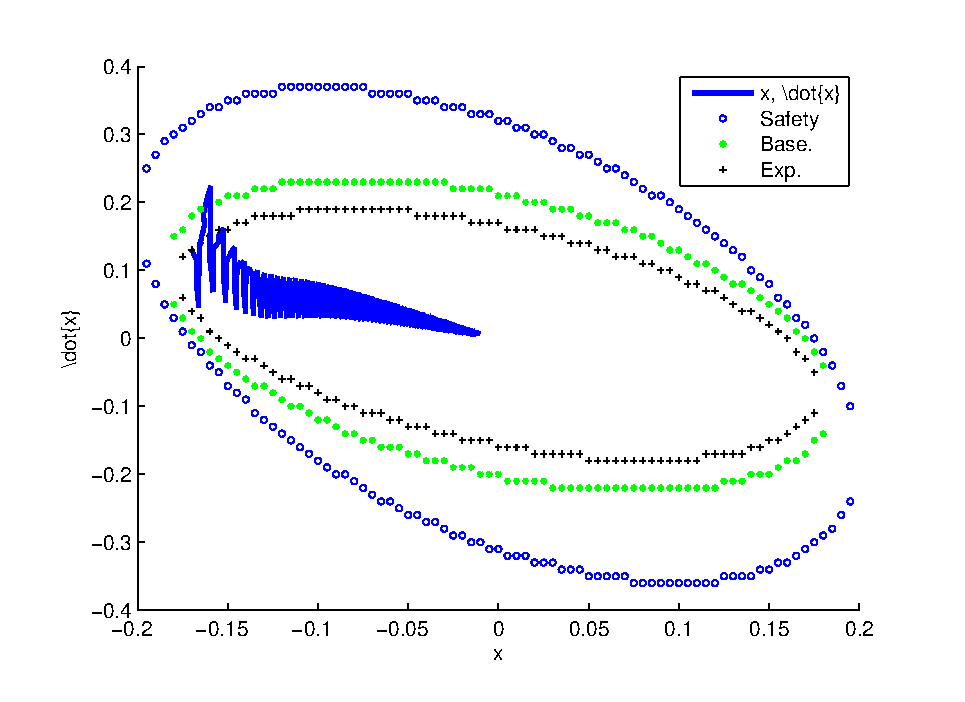
\includegraphics[width=250pt]{trajSwitchX}
\caption{Trajectory of $x$, $\dot{x}$ Switching Every $T_s$}\label{fig:trajSwitchX}
\end{figure}

\begin{figure}[htp]
\centering
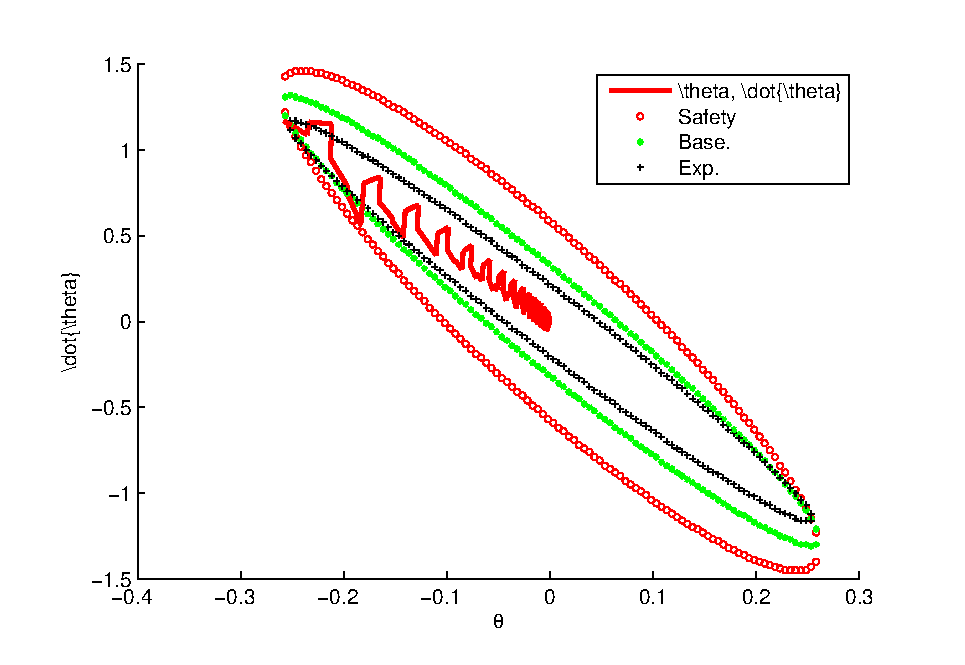
\includegraphics[width=250pt]{trajSwitchTheta}
\caption{Trajectory $\theta$, $\dot{\theta}$ Switching Every $T_s$}\label{fig:trajSwitchTheta}
\end{figure}

\begin{figure}[htp]
\centering
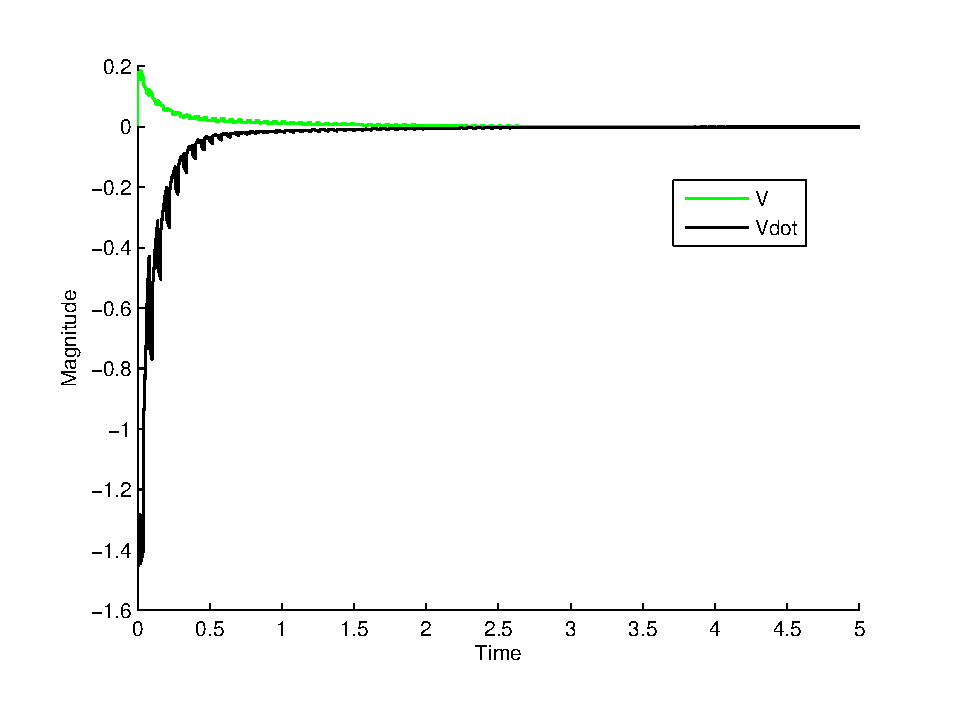
\includegraphics[width=250pt]{lyapSwitchReal}
\caption{Lyapunov Function for Switching Every $T_s$}\label{fig:lyapSwitchReal}
\end{figure}


% An example of a floating figure using the graphicx package.
% Note that \label must occur AFTER (or within) \caption.
% For figures, \caption should occur after the \includegraphics.
% Note that IEEEtran v1.7 and later has special internal code that
% is designed to preserve the operation of \label within \caption
% even when the captionsoff option is in effect. However, because
% of issues like this, it may be the safest practice to put all your
% \label just after \caption rather than within \caption{}.
%
% Reminder: the "draftcls" or "draftclsnofoot", not "draft", class
% option should be used if it is desired that the figures are to be
% displayed while in draft mode.
%
%\begin{figure}[!t]
%\centering
%\includegraphics[width=2.5in]{myfigure}
% where an .eps filename suffix will be assumed under latex, 
% and a .pdf suffix will be assumed for pdflatex; or what has been declared
% via \DeclareGraphicsExtensions.
%\caption{Simulation Results}
%\label{fig_sim}
%\end{figure}

% Note that IEEE typically puts floats only at the top, even when this
% results in a large percentage of a column being occupied by floats.


% An example of a double column floating figure using two subfigures.
% (The subfig.sty package must be loaded for this to work.)
% The subfigure \label commands are set within each subfloat command, the
% \label for the overall figure must come after \caption.
% \hfil must be used as a separator to get equal spacing.
% The subfigure.sty package works much the same way, except \subfigure is
% used instead of \subfloat.
%
%\begin{figure*}[!t]
%\centerline{\subfloat[Case I]\includegraphics[width=2.5in]{subfigcase1}%
%\label{fig_first_case}}
%\hfil
%\subfloat[Case II]{\includegraphics[width=2.5in]{subfigcase2}%
%\label{fig_second_case}}}
%\caption{Simulation results}
%\label{fig_sim}
%\end{figure*}
%
% Note that often IEEE papers with subfigures do not employ subfigure
% captions (using the optional argument to \subfloat), but instead will
% reference/describe all of them (a), (b), etc., within the main caption.


% An example of a floating table. Note that, for IEEE style tables, the 
% \caption command should come BEFORE the table. Table text will default to
% \footnotesize as IEEE normally uses this smaller font for tables.
% The \label must come after \caption as always.
%
%\begin{table}[!t]
%% increase table row spacing, adjust to taste
%\renewcommand{\arraystretch}{1.3}
% if using array.sty, it might be a good idea to tweak the value of
% \extrarowheight as needed to properly center the text within the cells
%\caption{An Example of a Table}
%\label{table_example}
%\centering
%% Some packages, such as MDW tools, offer better commands for making tables
%% than the plain LaTeX2e tabular which is used here.
%\begin{tabular}{|c||c|}
%\hline
%One & Two\\
%\hline
%Three & Four\\
%\hline
%\end{tabular}
%\end{table}


% Note that IEEE does not put floats in the very first column - or typically
% anywhere on the first page for that matter. Also, in-text middle ("here")
% positioning is not used. Most IEEE journals/conferences use top floats
% exclusively. Note that, LaTeX2e, unlike IEEE journals/conferences, places
% footnotes above bottom floats. This can be corrected via the \fnbelowfloat
% command of the stfloats package.


\section{Future Work}
This work began with the desire to prove stability of the Simplex architecture switching controller in this case study.  However, we have not quite yet proved this, although progress has been made.  We theorize that the tolerable delay of the entire system is the minimum tolerable delay across all controllers, so that $\tau_{\sigma}=\tau_{ec}$.

We have begun looking at the small-gain result in the system with minor nonlinearities that can be linearized, such as the $sin(\theta)$ term which for small $\theta$ can be linearized to $\theta$.  Some derivation in this direction is as follows.  Consider the nonlinear model,

\begin{equation}
\dot{X}=f\left(X,u\right)
\end{equation} We can then describe the equations of motion for the plant as 

\begin{equation}
\left(m+M\right)\ddot{x}+\frac{1}{2}ml\cos\left(\theta\right)\ddot{\theta}-\frac{1}{2}ml\sin\left(\theta\right)\dot{\theta}^2=F-f_c
\end{equation}

\begin{equation}
\frac{1}{2}ml\mathsf{\theta}\ddot{x}+\frac{1}{3}ml^2\ddot{\theta}-\frac{1}{2}mgl\sin\left(\theta\right)=-f_p
\end{equation} Skimming over the details of the motor model, we can achieve the entire system model including motor dynamics

\begin{equation}
\ddot{x}=\frac{1}{D}\left[\frac{1}{3}ml^2\left(B_lV_a-f_c-C_1\right)+\frac{1}{2}ml\cos\theta\left(f_p+C_2\right)\right]
\end{equation}

\begin{equation}
\ddot{\theta}=\frac{1}{D}\left[-\frac{1}{2}ml\cos\theta\left(B_lV_a-f_c-C_1\right)-\bar{M}\left(f_p+C_2\right)\right]
\end{equation} where $D=\frac{1}{3}\bar{M}ml^2-\frac{1}{4}m^2l^2\cos^2\left(\theta\right)$, $\bar{M}=\frac{m+M+(K_gJ_m)}{r^2}$, $C_1=\bar{B}\dot{x}-\frac{1}{2}ml\sin\left(\theta\right)\dot{\theta}^2$, $C_2=-\frac{1}{2}mgl\sin\left(\theta\right)$, $\bar{B}=\frac{K_gB_m}{r^2}+\frac{K_g^2K_iK_b}{r^2R_a}$, and $B_l=\frac{K_gK_i}{rR_a}$.  The immediate next step is to derive a Lyapunov function for this system, and when considering the earlier form of $V=X^TPX$, one could interchange the bounds on the $\theta$ states with $a\cos\left(\theta\right)$ where $a$ is some constant (since now we are considering $\sin\left(\theta\right)$).  After checking that this $P$ is positive definite and satisfies $A^TP+PA=-Q$, we could then proceed with our analysis as before.

With either the nonlinear or linearized models, there seem to be several areas to investigate in terms of common Lyapunov functions, multiple Lyapunov functions, and dwell-time, all seen in \cite{LiberzonSSC2003}.  So another step is an investigation of the average-dwell time (ADT) of the switching between the safety, baseline, and experimental controllers to see if ADT relates to the small-gain delay and stability regions.  Given the large length of time between switches, $T_s=20$ms, it may be possible to find a dwell-time less than this to prove overall stability.

As far as long-term future work, for the verification of the model to most closely match the real system, analyzing both the measurement and actuation errors from quantization and delay (from analog-to-digital conversion and digital-to-analog conversion, respectively) would provide a complete answer of the disturbances introduced by these non-ideal blocks.  There is also another avenue potentially to follow in the area of software verification through the co-stability concept.

\section{Conclusion}
This case study of the inverted pendulum with a controller following the Simplex architecture displays that recent results in small-gain theorems can be useful in practical systems.  Since the maximum tolerable delay found for stability was less than the control period length, it was necessary to project the state forward to the next control cycle to guarantee stability.  Thus, this work has shown that the system is still stable even with small delays introduced by measurement, so a stronger stability result was found for this system.

\section*{Acknowledgment}
The author would like to thank Sayan Mitra for helpful commentary and feedback throughout the work, Qixin Wang for guidance in working with the real inverted pendulum system, Lui Sha for revealing details not seen in his earlier work, and Daniel Liberzon for providing a clear description of small-gain theorems.


% trigger a \newpage just before the given reference
% number - used to balance the columns on the last page
% adjust value as needed - may need to be readjusted if
% the document is modified later
%\IEEEtriggeratref{8}
% The "triggered" command can be changed if desired:
%\IEEEtriggercmd{\enlargethispage{-5in}}

% references section

% can use a bibliography generated by BibTeX as a .bbl file
% BibTeX documentation can be easily obtained at:
% http://www.ctan.org/tex-archive/biblio/bibtex/contrib/doc/
% The IEEEtran BibTeX style support page is at:
% http://www.michaelshell.org/tex/ieeetran/bibtex/
\bibliographystyle{IEEEtran}
% argument is your BibTeX string definitions and bibliography database(s)
\bibliography{IEEEabrv,conference}
%
% <OR> manually copy in the resultant .bbl file
% set second argument of \begin to the number of references
% (used to reserve space for the reference number labels box)
%\begin{thebibliography}{1}

%\bibitem{IEEEhowto:kopka}
%H.~Kopka and P.~W. Daly, \emph{A Guide to \LaTeX}, 3rd~ed.\hskip 1em plus
%  0.5em minus 0.4em\relax Harlow, England: Addison-Wesley, 1999.

%\end{thebibliography}




% that's all folks
\end{document}
